%--------------------------------------------------------------------
%--- Licence
%--------------------------------------------------------------------

% An Introduction to LaTeX
%
% This work is a derivative of
%   "LaTeX: More Than Just Academic Papers and Journals"
% by Lim Lian Tze, used under a CC-BY-NC-SA 3.0 licence.
%
% Link: http://liantze.penguinattack.org/latextypesetting.html
%
% This work is licenced under a CC-BY-NC-SA 4.0 licence 
% by Martins Bruveris.

%--------------------------------------------------------------------
%--- Choose compilation mode
%--------------------------------------------------------------------

% Full presentation (with overlays, animated bullet items etc)
% \documentclass[xcolor={x11names,svgnames,dvipsnames},
%                usepdftitle=false]{beamer}

% Transparency mode (no overlays)
\documentclass[xcolor={x11names,svgnames,dvipsnames},
                  usepdftitle=false, trans]{beamer}

% n-up handout mode
% \documentclass[xcolor={x11names,svgnames,dvipsnames},
%                usepdftitle=false, handout]{beamer}

%--------------------------------------------------------------------
%--- Beamer setup
%--------------------------------------------------------------------

\usepackage{pgfpages}  % Needed here for handout specification

% For presentation mode, use simple slides with red titles
\mode<beamer|trans>{
\useoutertheme{default}
\useinnertheme[shadow,outline]{chamfered}
\usecolortheme{beaver}
}

% No navigation symbols
\setbeamertemplate{navigation symbols}{}

% In case of continued frames, don't use roman numbering
\setbeamertemplate{frametitle continuation}[from second][(cont'd)]

% Normal and small text sans serif, remaining in serif
\usefonttheme[stillsansseriftext,stillsansserifsmall]{serif}

% Set margins
\setbeamersize{text margin left=0.5cm,text margin right=0.5cm} 

% Setup for handouts
\mode<handout>{
\useoutertheme{default}
\useinnertheme[shadow,outline]{chamfered}

% Use black and white mostly
\setbeamercolor{structure}{fg=black}
\setbeamercolor{alerted text}{fg=black}

% % 2 slides per page
% \pgfpagesuselayout{2 on 1}[a4paper, border shrink=10mm]
% \pgfpageslogicalpageoptions{1}{border code=\pgfstroke}
% \pgfpageslogicalpageoptions{2}{border code=\pgfstroke}

% 4 slides per page
\pgfpagesuselayout{4 on 1}[a4paper, landscape, border shrink=10mm]
\pgfpageslogicalpageoptions{1}{border code=\pgfstroke}
\pgfpageslogicalpageoptions{2}{border code=\pgfstroke}
\pgfpageslogicalpageoptions{3}{border code=\pgfstroke}
\pgfpageslogicalpageoptions{4}{border code=\pgfstroke}
}

% Repeat table of contents at the beginning of each section
\mode<beamer|trans>{\AtBeginSection[]{%
\begin{frame}
\frametitle{Contents}
\tableofcontents[currentsection]
\end{frame}}}

% Centered, variable width block
% Source: tex.stackexchange.com/questions/12550
\newenvironment<>{cvarblock}[2][\textwidth]{%
  \begin{center}
  \begin{minipage}{#1}
  % The -2.5pt is avoid overfull hbox errors; Has to do with blocks
  \setlength{\textwidth}{\textwidth-2.5pt}
  % Required to itemize respect the width of block
  \setlength{\linewidth}{\textwidth}       
  \begin{actionenv}#3%
    \def\insertblocktitle{#2}%
    \par%
    \usebeamertemplate{block begin}
}{
    \par%
    \usebeamertemplate{block end}%
  \end{actionenv}
  \end{minipage}
  \end{center}
}

\newenvironment<>{varblock}[2][\textwidth]{%
  % The -2.5pt is avoid overfull hbox errors; Has to do with blocks
  \setlength{\textwidth}{\textwidth-2.5pt}
  % Required to itemize respect the width of block
  \setlength{\linewidth}{\textwidth}       
  \begin{actionenv}#3%
    \def\insertblocktitle{#2}%
    \par%
    \usebeamertemplate{block begin}
}{
    \par%
    \usebeamertemplate{block end}%
  \end{actionenv}
}

%--------------------------------------------------------------------
%--- Loading of packages
%--------------------------------------------------------------------

\usepackage[utf8]{inputenc}
\usepackage[T1]{fontenc}
\usepackage{microtype}

\usepackage{libertine}              % LinuxBiolinum Font
\usepackage[scaled=.77]{beramono}   % Typewriter font
\usepackage[T1,safe]{tipa}          % Phonetic alphabet

\usepackage[british]{babel}
\usepackage{textcomp}            % Is necessary, not entirely sure why
\usepackage{relsize}             % \textsmaller, etc.
\usepackage{tikz}
\usepackage{ccicons}             % CC licence symbols
\usepackage{upgreek}             % Greek letters for `textmode'
\usepackage{adforn}              % Ornaments on title page
\usepackage{adjustbox}           % For easy clipping of images
\usepackage{substitutefont}      % \substitutefont (see below, T3 and IPA)
\usepackage{multicol,multirow}   % For large cells in tables; see Questions slide
\usepackage{booktabs}            % Nicely spaced tables
\usepackage{hologo}              % \LaTeX logo, bookmark friendly
  \usepackage{tabularx}          % Seems necessary for \hologo in \item[...]
\usepackage{listings}            % \lstlistings for source code

% Packages used for domain specific tasks
\usepackage[version=3]{mhchem}
\usepackage{chemfig}
\usepackage[detect-all]{siunitx}
\usepackage[siunitx]{circuitikz}
\usepackage{smartdiagram}
\usepackage{pgfplots}
\pgfplotsset{compat=1.13}
\usepackage{cwpuzzle}
\usepackage{gchords,guitar}
\usepackage{expex,qtree}
\usepackage[skaknew]{chessboard,skak}
\usepackage{pgfgantt}
\usepackage[all]{xy}
% \usepackage{pstricks,pst-barcode} % For barcodes, not compiled at the moment
% \usepackage{auto-pst-pdf}         % Ditto

% Apparently unused packages; from original version
% \usepackage{marvosym}
% \usepackage{booktabs}
% \usepackage{bookmark}
% \usepackage{bytefield}
% \usepackage{texshade}

%--------------------------------------------------------------------
%--- Global setup
%--------------------------------------------------------------------

% Microtype setup
\SetTracking{encoding=*}{-39}

% No boundary around frameboxes
\setlength\fboxsep{0pt}

\urlstyle{same}  % URLs not in typewriter font

% This command fills available vertical space so text can appear at
% the bottom of the page.
\newcommand{\btVFill}{\vskip0pt plus 1filll}

% Phonetic alphabet uses T3 encoding, but font loaded by libertine
% is only available as T1. Substitute Computer Modern instead.
\substitutefont{T3}{LinuxBiolinumT-TLF}{cmr}

%--------------------------------------------------------------------
%--- Listings setup
%--------------------------------------------------------------------

\lstset{
  upquote,
  keepspaces=true,
  columns=spaceflexible,
  breaklines=true,
  breakindent=0pt,
  xleftmargin=0pt, 
  xrightmargin=6pt,
  language=[LaTeX]TeX, 
  basicstyle=\ttfamily\scriptsize,
  texcsstyle=*\bfseries\color{Maroon},
  commentstyle=\sffamily\itshape\smaller\color{SeaGreen4},
  emphstyle=\bfseries\color{RoyalBlue3},escapechar={:},
  emphstyle={[2]{\bfseries\color{Sienna2}}},
  postbreak=\mbox{{\smaller\color{gray}$\hookrightarrow$}}
}

\mode<handout>{
   \lstset{
   texcsstyle=*\bfseries, commentstyle=\sffamily\itshape\smaller,
   emphstyle=\bfseries,escapechar={:},
   emphstyle={[2]{\bfseries}},
   emphstyle={[3]{\bfseries}},
   postbreak=\mbox{{\smaller$\hookrightarrow$}}
   }
}

% Changes hyphens into minus signs for tt font.
\makeatletter
\lst@CCPutMacro\lst@ProcessOther {"2D}{\lst@ttfamily{-{}}{-{}}}
\@empty\z@\@empty
\makeatother

%--------------------------------------------------------------------
%--- Title
%--------------------------------------------------------------------

\title{An Introduction to \LaTeX}
\subtitle{
  \makebox[\linewidth]{%
  \hrulefill\quad
  \raisebox{-.8ex}{%   % To vertically center the horizontal lines
    \adforn{21}\quad\adforn{11}\quad\adforn{49}}
  \quad\hrulefill}
}

\author[Martins Bruveris]{%
\rmfamily Martins Bruveris \\
\href{http://www.brunel.ac.uk/~mastmmb}{%
\textsmaller{\url{http://www.brunel.ac.uk/~mastmmb}}}
}

\date{%
\rmfamily February \oldstylenums{13}, \oldstylenums{2017}
}

\titlegraphic{%

\includegraphics[width=.3\textwidth]{images/TFZsuperellipse-crop} \\
\tiny Illustration by Duane Bibby
}

\hypersetup{%
  pdftitle={An Introduction to LaTeX},
  pdfauthor={Martins Bruveris},
  pdfkeywords={latex, introduction, features, typesetting}
}

%--------------------------------------------------------------------
%--- Begin slides
%--------------------------------------------------------------------

\begin{document}
\begin{frame}[plain]
\maketitle
\end{frame}

% If we want a table of contents
\begin{frame}
\frametitle{Contents}
\tableofcontents
\end{frame}

% What is LateX?
% !TEX root=talk.tex
\section[Introduction]{What are \TeX, \LaTeX\ and Friends?}

%--------------------------------------------------------------------
%--- The FYP
%--------------------------------------------------------------------

\begin{frame}[fragile]
\setlength{\fboxsep}{0.333em}
\frametitle{The Final Year Project}
Is $50$--$70$ pages long and contains
\pause

\begin{itemize}
\item Mathematical equations\hspace{1em}\framebox{$\displaystyle\int_{-\infty}^\infty e^{-x^2} \,\mathrm{d}x = \sqrt{\pi}$}
\pause

\item Graphs
\hspace{18em}\raisebox{0pt}[0pt][0pt]{\framebox{
\begin{tikzpicture}[scale=0.5, baseline=1.25]
  \draw[->,>={Stealth[length={4pt}]}] (-2,0) -- (2,0);
  \draw[->,>={Stealth[length={4pt}]}] (0,-.5) -- (0,2);

  \clip (-2,-.5) rectangle (2,2);

  \draw plot[parametric, domain=-2:2, samples=100] function {t, t**3-t+0.5};
\end{tikzpicture}
}}
\pause

\item Tables
\hspace{1em}\raisebox{0em}[2em][2em]{
\framebox{
\begin{tabular}{lccc}
$x$ & 0 & 1 & 2 \\ \midrule
$y$ & 0.5 & 0.5 & 7.5
\end{tabular}}}
\pause

\item Source code
\hspace{0.5em}\begin{minipage}{8em}
\begin{lstlisting}[frame=single,language=matlab,lineskip=-2pt,
basicstyle=\ttfamily,
commentstyle=\upshape\sffamily\small\color{SeaGreen4},keepspaces=true,
keywordstyle=\bfseries\color{Maroon},stringstyle=\rmfamily\color{Sienna2}]
if x > 0
    y = sqrt(x);
end
\end{lstlisting}
\end{minipage}
\pause

\item References and a bibliography
\hspace{2em}\raisebox{1em}[0em][2em]{\framebox{
\begin{minipage}{13em}
\textsmaller{\rmfamily\noindent
See [1, Theorem~1.2.6] for a proof.
\smallskip

[1] S.~Abbott. \emph{Understanding Analysis}. \\
Undergraduate Texts in Mathematics. Springer, New York, 2015.}
\end{minipage}}}
\end{itemize}
\end{frame}

% %--------------------------------------------------------------------
% %--- Ever Worried about These?
% %--------------------------------------------------------------------

% \begin{frame}
% \frametitle{Ever Worried about These?}
% \begin{itemize}
% \item<2-12,13> Is my introduction good enough?
% \item<3-12,14|alert@14|trans:alert@1|handout:alert@1> My math equations don't display correctly.
% \item<4-12,13> Should this discussion go into this section or that one?
% \item<5-12,14|alert@14|trans:alert@1|handout:alert@1> What formatting did I use for my subsection headings again?
% \item<6-12,14|alert@14|trans:alert@1|handout:alert@1> My section/figure/page numbering has gone all wrong!
% \item<7-12,13> Should I split this section into two?
% \item<8-12,14|alert@14|trans:alert@1|handout:alert@1> My citation formatting got inconsistent.
% \item<9-12,14|alert@14|trans:alert@1|handout:alert@1> My citations and bibliography aren't synchronised!
% \item<10-12,13> What results should I put in this table?
% \item<11-12,14|alert@14|trans:alert@1|handout:alert@1> Oops, I forgot to update the table of contents.
% \item<12,14|alert@14|trans:alert@1|handout:alert@1> Should I think some more about the conclusions section?
% \end{itemize}
% \end{frame}

%--------------------------------------------------------------------
%--- Tex, LaTeX, and Friends
%--------------------------------------------------------------------

\begin{frame}<1>[label=texNfriends]
\frametitle{What are \TeX\ and \LaTeX,\ and Friends?}

\begin{description}
\item<1>[\TeX] 
\begin{itemize}
\item From Greek $\uptau\upepsilon\upchi$. \\
Abbreviation of $\uptau\upepsilon\upchi\upnu\upeta$, meaning \emph{art} or \emph{craft}.
\item \textsmaller{ASCII} \texttt{TeX}, \textsmaller{\textipa{/tEx/}, \textipa{/tEk/}}.
\item A \structure{computer typesetting system} created by Donald Knuth
for `the creation of beautiful books'. First release 1978. (39 years ago!)
\end{itemize}


\item<2>[\LaTeX]
\begin{itemize}
\item A shortening of `Lamport-\TeX'.
\item \textsmaller{ASCII} \texttt{LaTeX}, \textsmaller{\textipa{/"leItEx/}, \textipa{/"leItEk/}, \textipa{/"lA:tEx/}, \textipa{/"lA:tEk/}}.
\item A \structure{document preparation system} by Leslie Lamport. First release 1985.
	\end{itemize}

\item <3>[Friends]
\begin{itemize}
\item \structure{Bib\TeX}, \structure{Biber}, \structure{MakeIndex}, \ldots
\item \url{http://www.ctan.org/what_is_tex.html}
\end{itemize}
\end{description}
\end{frame}

%--------------------------------------------------------------------
%--- Knuth and Lamport
%--------------------------------------------------------------------

{\setbeamertemplate{background canvas}{\hskip-2em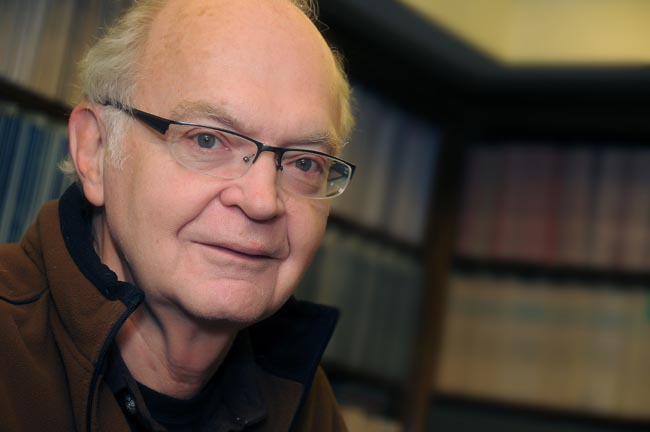
\includegraphics[height=\paperheight]{images/d_knuth_noticia}}
\setbeamercolor{itemize item}{fg=structure.fg!45}
\begin{frame}[plain,t]
\vfill
\hfill
\begin{minipage}{.42\textwidth}
\usebeamercolor[bg]{normal text}
\hspace{1em}\textbf{\large Donald Knuth (1938--)}
\begin{itemize}
\usebeamercolor[bg]{normal text}
\item American computer scientist, mathematician, and professor emeritus at Stanford University
\item Author of the multi-volume work \emph{The Art of Computer Programming}
\item ``Father of the analysis of algorithms''
\end{itemize}
\end{minipage}

\bigskip

\begin{quote}
\usebeamercolor[bg]{normal text}
``Science is what we understand well enough to explain to a computer. Art is everything else we do.''

\medskip

``If you optimize everything, you will always be unhappy.''
\end{quote}
\vspace*{-4\baselineskip}\null
\end{frame}}

\mode<beamer>{
  \againframe<2>{texNfriends}
}

{\setbeamertemplate{background canvas}{%
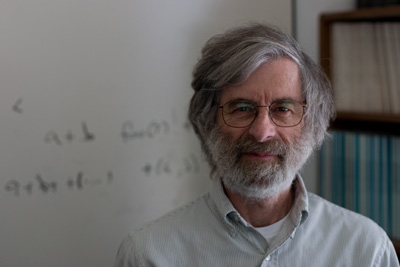
\includegraphics[height=\paperheight]{images/lamport}}
\setbeamercolor{itemize item}{fg=structure.fg!45}
\begin{frame}[plain,t]
\vfill
\begin{minipage}{.45\textwidth}
\usebeamercolor[bg]{normal text}
\hspace{1em}\textbf{\large Leslie Lamport (1941--)}
\begin{itemize}
\usebeamercolor[bg]{normal text}
\item American computer scientist
\item Laid the foundations of the theory of distributed systems
\end{itemize}

\bigskip

\emph{
\usebeamercolor[bg]{normal text}
``A distributed system is one in which the failure of a computer you didn't even know existed can render your own computer unusable.''}
\end{minipage}
\end{frame}
}

\mode<beamer>{
  \againframe<3->{texNfriends}
}

%--------------------------------------------------------------------
%--- Typesetting and Word Processing
%--------------------------------------------------------------------

\begin{frame}
\frametitle{Typesetting and Word Processing}
\framesubtitle{Apples and Oranges}

\begin{columns}[T]
\begin{column}{.5\textwidth}
\textlarger{\structure{Word Processors}} \\
\textsmaller{Word, Google Docs, LibreOffice}
\begin{itemize}
\item What you see is what you get.
\item Content and layout are generated at the same time.
\item Local style adjustments are easier to make.
\end{itemize}
\end{column}

\onslide<3>
\begin{column}{.5\textwidth}
\textlarger{\structure{Typesetting Software}} \\
\textsmaller{\LaTeX, InDesign, Scribus}
\begin{itemize}
\item Separation of content and presentation.
\item Layout can be globally optimised.
\item Uniform style easier to realise.
\end{itemize}
\end{column}
\end{columns}

\onslide<2->
\begin{cvarblock}[0.82\textwidth]{}
\textbf{typesetting} \emph{n}. The activity of arranging printed text and images on the page when preparing a book, newspaper, etc. for printing.
\hfill\textsmaller{(Cambridge English Dictionary)}
\end{cvarblock}

\end{frame}

%--------------------------------------------------------------------
%--- Scalability
%--------------------------------------------------------------------

\begin{frame}
\frametitle{Scalability}
\bigskip

\centering
\begin{tikzpicture}
  %\draw[help lines,gray!20] (0,0) grid (6,4);
  %\draw[semithick] (0,0) rectangle (6,4);
  \draw[semithick,->,>=latex'] (-.5, 0) -- (6.5, 0);
  \draw[semithick,->,>=latex'] (0, -.5) -- (0,5);
  \draw[dashed,structure.fg!50!black,semithick] 
    (0, 0.2) parabola (3.5,4)
      node[above, font=\footnotesize, text=black]{Impossible to do} (3.5, 4);
  \node[left] at (3,3) {MS Word};
  \draw[structure.fg!50!black,semithick] (0, 1) parabola (6,3); 
  \node at (5.2,2) {\LaTeX};
  \node[below,font=\footnotesize] at (3,0) {Document complexity and size};
  \node[xshift=-8pt, yshift=4pt, font=\footnotesize, transform shape, rotate=90] 
    at (0,2.2) {Effort and time consumption};
\end{tikzpicture}

\begin{center}
Scalability of \LaTeX\ and Microsoft Word as a function of \\
document size and complexity.
\end{center}

\btVFill

\hfill
\textsmaller{
Redrawn from Marko Pinteric's original \structure{\href{http://www.pinteric.com/miktex.html}{(link)}}.}
\medskip

\end{frame}

%--------------------------------------------------------------------
%--- Example .tex File
%--------------------------------------------------------------------

% TODO: Add creation of first-en.pdf file & cropping automatic
% TODO: See original file for swapping languages example

\begin{frame}[fragile]
\frametitle{Example \texttt{.tex} File}
\setlength{\fboxsep}{.5em}

\begin{columns}[T]
\begin{column}{.48\textwidth}
\begin{beamerboxesrounded}[width=\linewidth]{}
\vspace{-1em}
\begin{lstlisting}[moretexcs={maketitle,tableofcontents,subsection},
emph={document,abstract,babel},
basicstyle={\ttfamily\footnotesize\lsstyle},lineskip=-2pt]
\documentclass[a4paper,11pt]{article}
\author{Martins Bruveris}
\title{An Introductory Paper}
\date{\today}
\usepackage[english]{babel}

\begin{document}
\maketitle
\tableofcontents

\begin{abstract}
This paper introduces\ldots
\end{abstract}

\section{Introduction}
We consider\ldots

\section{State of the Art}
We look at\ldots

\subsection{Document Formats}
There are many\ldots
\end{document}
\end{lstlisting}
\vspace{-1em}
\end{beamerboxesrounded}
\end{column}

\begin{column}{.48\textwidth}
\uncover<3>{%
\hfill\fcolorbox{black}{white}{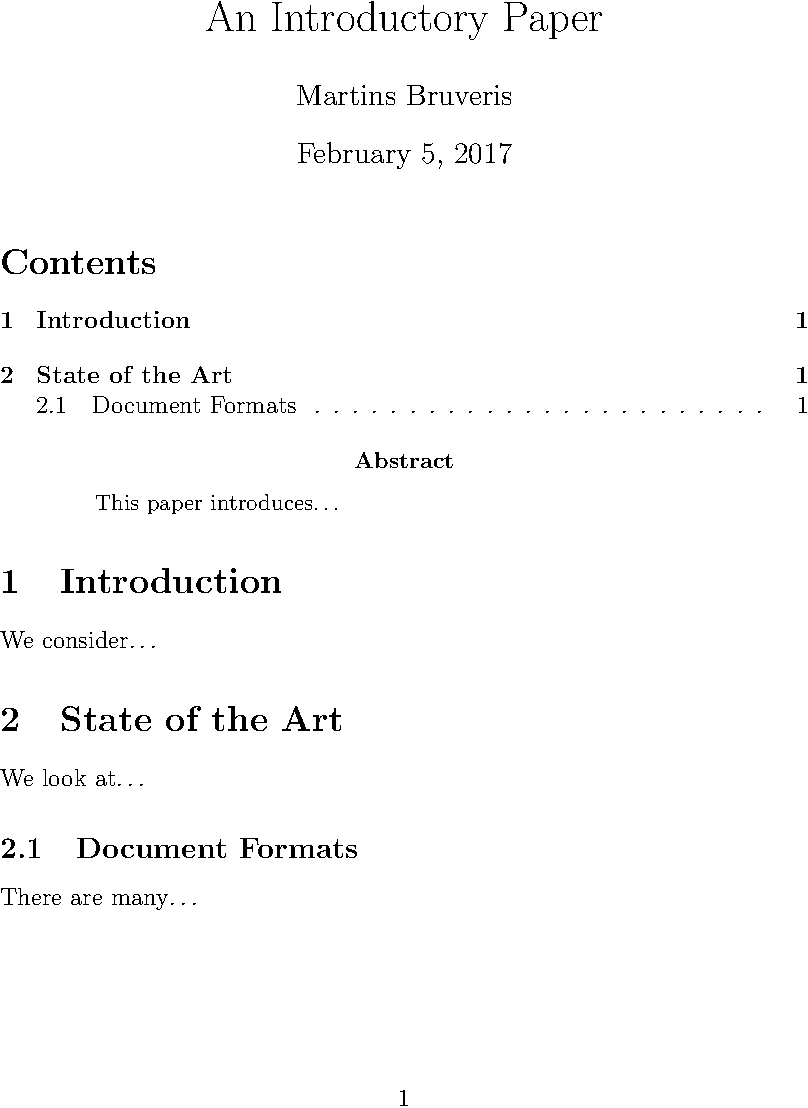
\includegraphics[width=0.94\linewidth]{examples/first-en}}
}
\end{column}
\end{columns}

\uncover<2->{%
\begin{tikzpicture}[remember picture,overlay]
\node[single arrow,fill=DarkSeaGreen,font=\ttfamily\bfseries,xshift=-1em] at (current page.center) {pdflatex};
\end{tikzpicture}
}

\end{frame}

%--------------------------------------------------------------------
%--- Module structure
%--------------------------------------------------------------------

\begin{frame}
\frametitle{Module Structure}

\begin{description}
\setlength\labelwidth{8.5em}
\setlength\itemindent{3em}
\item[Lecture]
Introduction to \LaTeX\ (happening right now)
\pause\medskip

\item[Labs]
Three computer labs for each group (W21--23) \\
\hspace{\itemindent}Mon, Tue or Thu 17--19 in HALB 213
\pause\medskip

\item[Assignment]
Preparing a document, about two pages long \\
\hspace{\itemindent} Thematically connected to MA2895 assignment \\
\hspace{\itemindent} Due 3 April 2017 (TBC)
\pause\medskip

\item[Assessment]
Contributes 20\% towards MA2812

\end{description}

\end{frame}

%--------------------------------------------------------------------
%--- Where Do I Get It?
%--------------------------------------------------------------------

\begin{frame}
\frametitle{Where Do I Get It?}
\begin{description}
\setlength\labelwidth{8.5em}
\setlength\itemindent{3em}
\item[Online]
ShareLaTeX (\url{www.sharelatex.com}) \\ 
\hspace{\itemindent}Overleaf (\url{www.overleaf.com})
\pause
\medskip
\item[Windows] Mik\TeX, \TeX Live
\item[Linux] \TeX Live
\item[Mac OS X] Mac\TeX\ (based on \TeX Live)
\pause
\medskip
\item[Editors]
TeXmaker, TeXworks, TeXstudio, emacs \\
\hspace{\itemindent}(Mac OS X) TeXShop
\pause
\medskip
\item[\hologo{LaTeX} Packages] Use Mik\TeX\ or \TeX Live's package manager
\pause
\medskip
\item[Documentation] 
(Online) \url{http://texdoc.net/pkg/<package name>}\\
\hspace{\itemindent}(\TeX Live) \texttt{\$ texdoc <package name>}\\
\hspace{\itemindent}(Mik\TeX) \texttt{\$ mthelp <package name>}
\end{description}
\end{frame}

%--------------------------------------------------------------------
%--- Where Can I Find Help?
%--------------------------------------------------------------------

\begin{frame}
\frametitle{Where Can I Find Help?}

\begin{description}
\setlength\labelwidth{7em}
\setlength\itemindent{1em}
\item[Online]
Search the internet \\
\hspace{\itemindent}%
\textsmaller{E.g. use `latex add table of contents' in your favorite search engine.} \\
\hspace{\itemindent}\TeX\ Stack Exchange 
\textsmaller{(\url{http://tex.stackexchange.com})} \\
\hspace{\itemindent}The \LaTeX\ Wikibook 
\textsmaller{ (\url{http://en.wikibooks.org/wiki/latex})}
\medskip
\pause

\item[Books]
George Graetzer, \emph{Practical \LaTeX}. Springer, 2014. \\
\hspace{\itemindent}\textsmaller{Electronic version available through the library.
\href{http://lib.myilibrary.com/Open.aspx?id=644795&src=0}{%
{\usebeamercolor[fg]{description item} (Link)}}} \\
\hspace{\itemindent}%
Helmut Kopka, Patric W.~Daley, \emph{Guide to \LaTeX}. \\
\hspace{\itemindent}Fourth Edition. Addison-Wesley, 2004. \\
\hspace{\itemindent}\textsmaller{Electronic version available through the library.
\href{http://lib.myilibrary.com/Open.aspx?id=243269&src=0}{%
{\usebeamercolor[fg]{description item} (Link)}}} \\
\medskip
\pause

\item[Other]
\LaTeX\ Cheat Sheet 
\href{https://wch.github.io/latexsheet/}{%
{\usebeamercolor[fg]{description item} \textsmaller{(Link)}}} \\
\hspace{\itemindent}The Not So Short Introduction to \LaTeXe
\href{http://tug.ctan.org/info/lshort/english/lshort.pdf}{%
{\usebeamercolor[fg]{description item} \textsmaller{(Link)}}} \\
\hspace{\itemindent}The ShareLaTeX Documentation
\href{https://www.sharelatex.com/learn}{%
{\usebeamercolor[fg]{description item} \textsmaller{(Link)}}} \\
\hspace{\itemindent}Overleaf \LaTeX Tutorial
\href{https://www.overleaf.com/latex/learn/free-online-introduction-to-latex-part-1}{%
{\usebeamercolor[fg]{description item} \textsmaller{(Link)}}}
\end{description}
\end{frame}

%--------------------------------------------------------------------
%--- Why use LaTeX
%--------------------------------------------------------------------

\begin{frame}
\frametitle{Why?}
\framesubtitle{From \url{http://www.ctan.org/what_is_tex.html}}
\begin{columns}[T]
\begin{column}{.48\textwidth}
\begin{varblock}<1->{Output Quality}
\begin{itemize}
\item Professional quality output.
\item It knows typesetting.
\end{itemize}
\end{varblock}

\begin{varblock}<2->{Superior Engineering}
\begin{itemize}
\item It's fast.
\item It's stable.
\item It's extensible.
\item Plain text input.
\item Many output types.
\end{itemize}
\end{varblock}
\end{column}

\begin{column}{.48\textwidth}
\begin{varblock}<3->{Freedom}
\begin{itemize}
\item It's free.
\item It runs anywhere.
\end{itemize}
\end{varblock}

\begin{varblock}<4->{Popularity}
\begin{itemize}
\item It's standard in academia and science.
\end{itemize}
\end{varblock}
\end{column}
\end{columns}
\end{frame}

%%% Local Variables:
%%% TeX-master: "talk"
%%% End:


% What document types are possible
% !TEX root=talk.tex

\section{Document Types}

\begin{frame}[fragile]
\frametitle{Article -- The Basic Document}

\begin{columns}
\begin{column}{.4\textwidth}
\begin{beamerboxesrounded}[width=\linewidth]{}
\begin{lstlisting}[moretexcs={chapter,subsection,maketitle}, basicstyle={\ttfamily}, emph={article}]
\documentclass{article}
\author{...}
\title{...}

\begin{document}
\maketitle
\section{...}
...
\subsection{...}
\end{document}
\end{lstlisting}
\end{beamerboxesrounded}
\end{column}
\begin{column}{.58\textwidth}
\centering
\fcolorbox{black}{white}{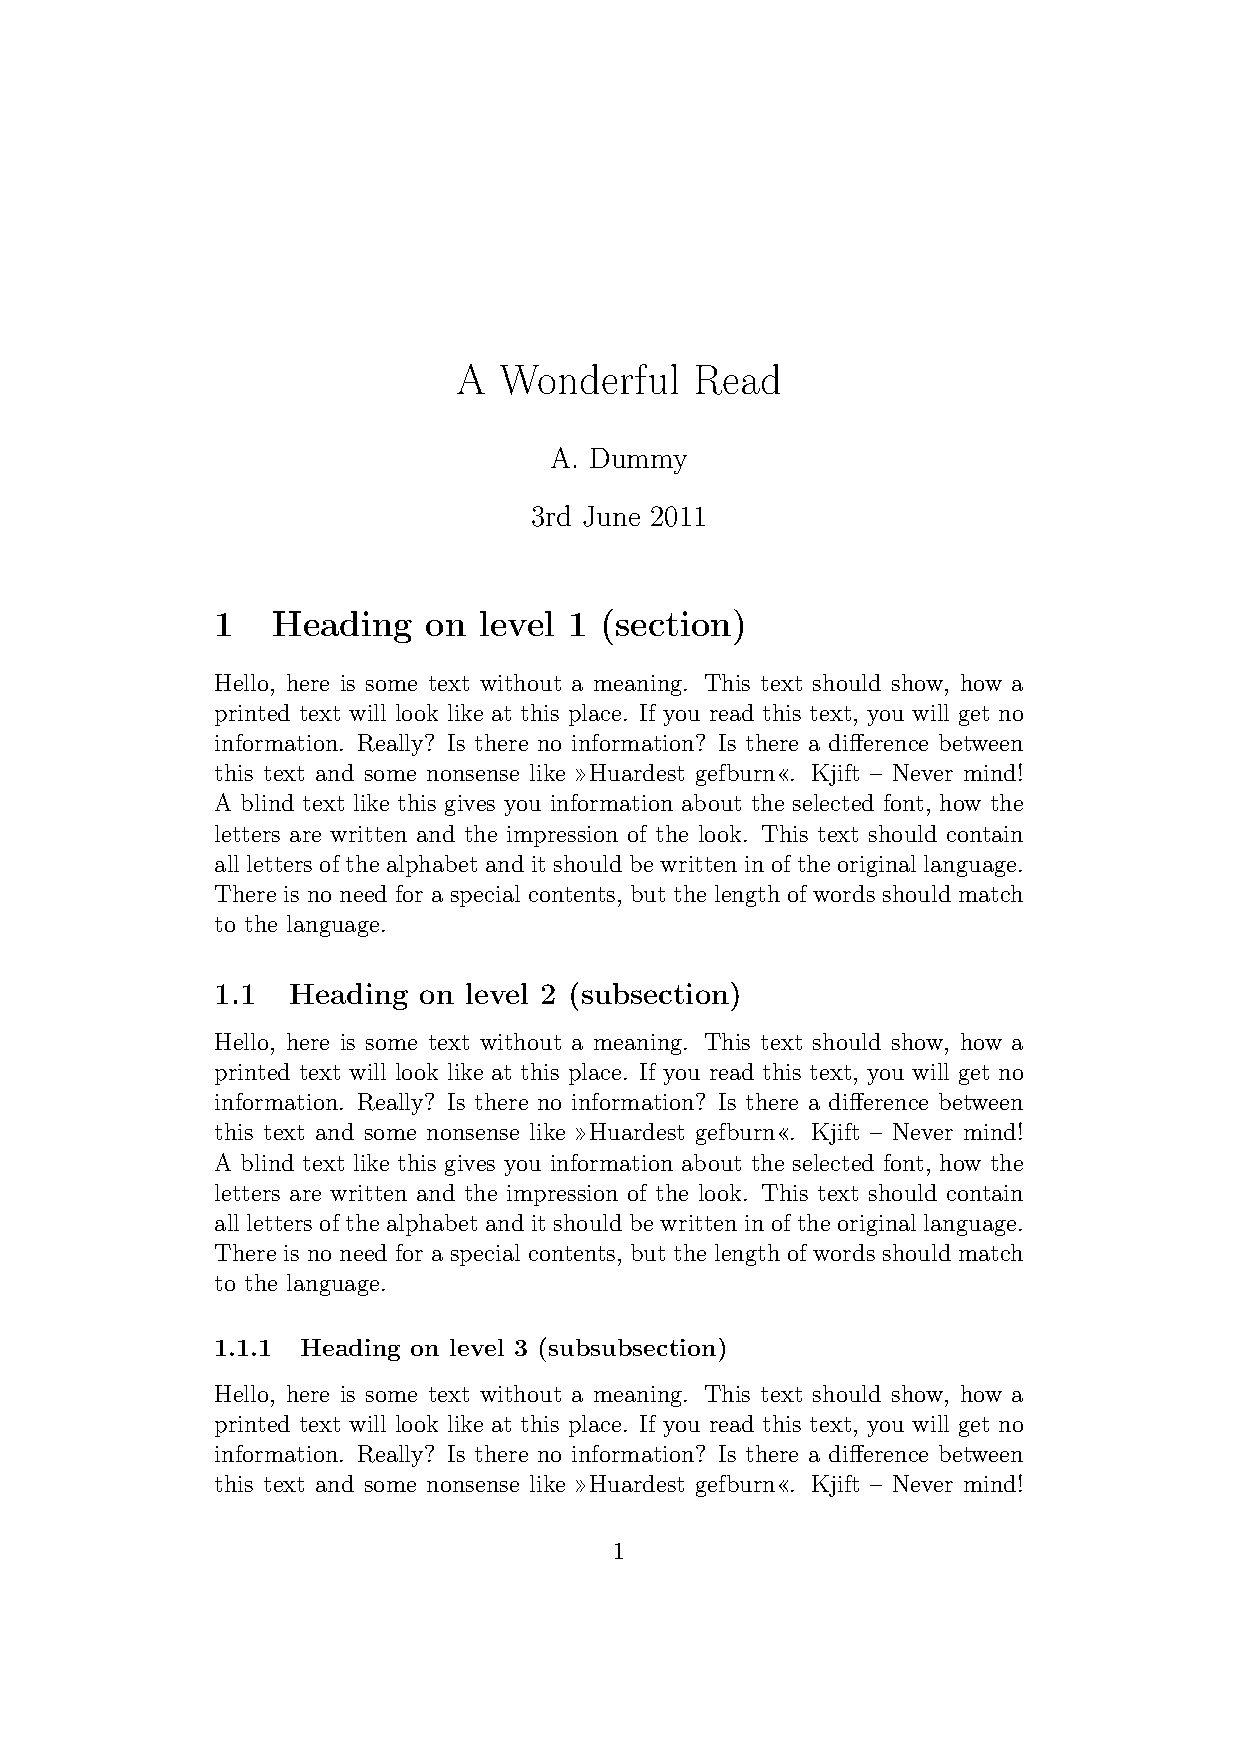
\includegraphics[width=.4\linewidth,page=1]{examples/basicarticle}}
\fcolorbox{black}{white}{\includegraphics[width=.4\linewidth,page=2]{examples/basicarticle}}
\fcolorbox{black}{white}{\includegraphics[width=.4\linewidth,page=3]{examples/basicarticle}}
\fcolorbox{black}{white}{\includegraphics[width=.4\linewidth,page=4]{examples/basicarticle}}
\end{column}
\end{columns}
\end{frame}




\begin{frame}[fragile]
\lstset{basicstyle=\ttfamily}
\frametitle{Some Features of \LaTeX}
\begin{itemize}
\item<+> Automatic generation of \structure{cross-referencing labels}:\\
\lstinline|\section{Introduction}\label{sec:intro}|\\
\lstinline|... We saw in section \ref{sec:intro}...|
\item<+> Automatic generation of \structure{lists}:\\
\lstinline[texcs={tableofcontents}]|\tableofcontents|, \lstinline[texcs={listoffigures}]|\listoffigures|,  \lstinline[texcs={listoftables}]|\listoftables|
\item<+> Automatic generation of \structure{bibliographies} and \structure{indices}:\\
\lstinline|\cite{Knuth:1976}...\bibliography{references.bib}|\\
\lstinline[moretexcs={printindex}]|...the Linux kernel\index{Linux!kernel}... \printindex|\\
\item<+> Fully \structure{hyperlinked} \textsmaller{PDF} with bookmarks: \lstinline|\usepackage{hyperref}|
\item<+> Inclusion of selected pages from other \textsmaller{PDF}s\\(while inserting new page headers/footers!)\\
\lstset{basicstyle=\ttfamily\footnotesize,moretexcs={includepdf}}
\lstinline|\usepackage{pdfpages}|\\
\lstinline|\includepdf[pages={1,3-5,8},pagecommand=\thispagestyle{plain}]{file.pdf}|
\item<+> Quick \structure{language-switching} with \texttt{babel}
\end{itemize}
\end{frame}


\begin{frame}[fragile]
\frametitle{Your Final Year Project}

\bigskip
\bigskip

A template for a university thesis.

\vskip.5em

\begin{center}
\fcolorbox{black}{white}{%
  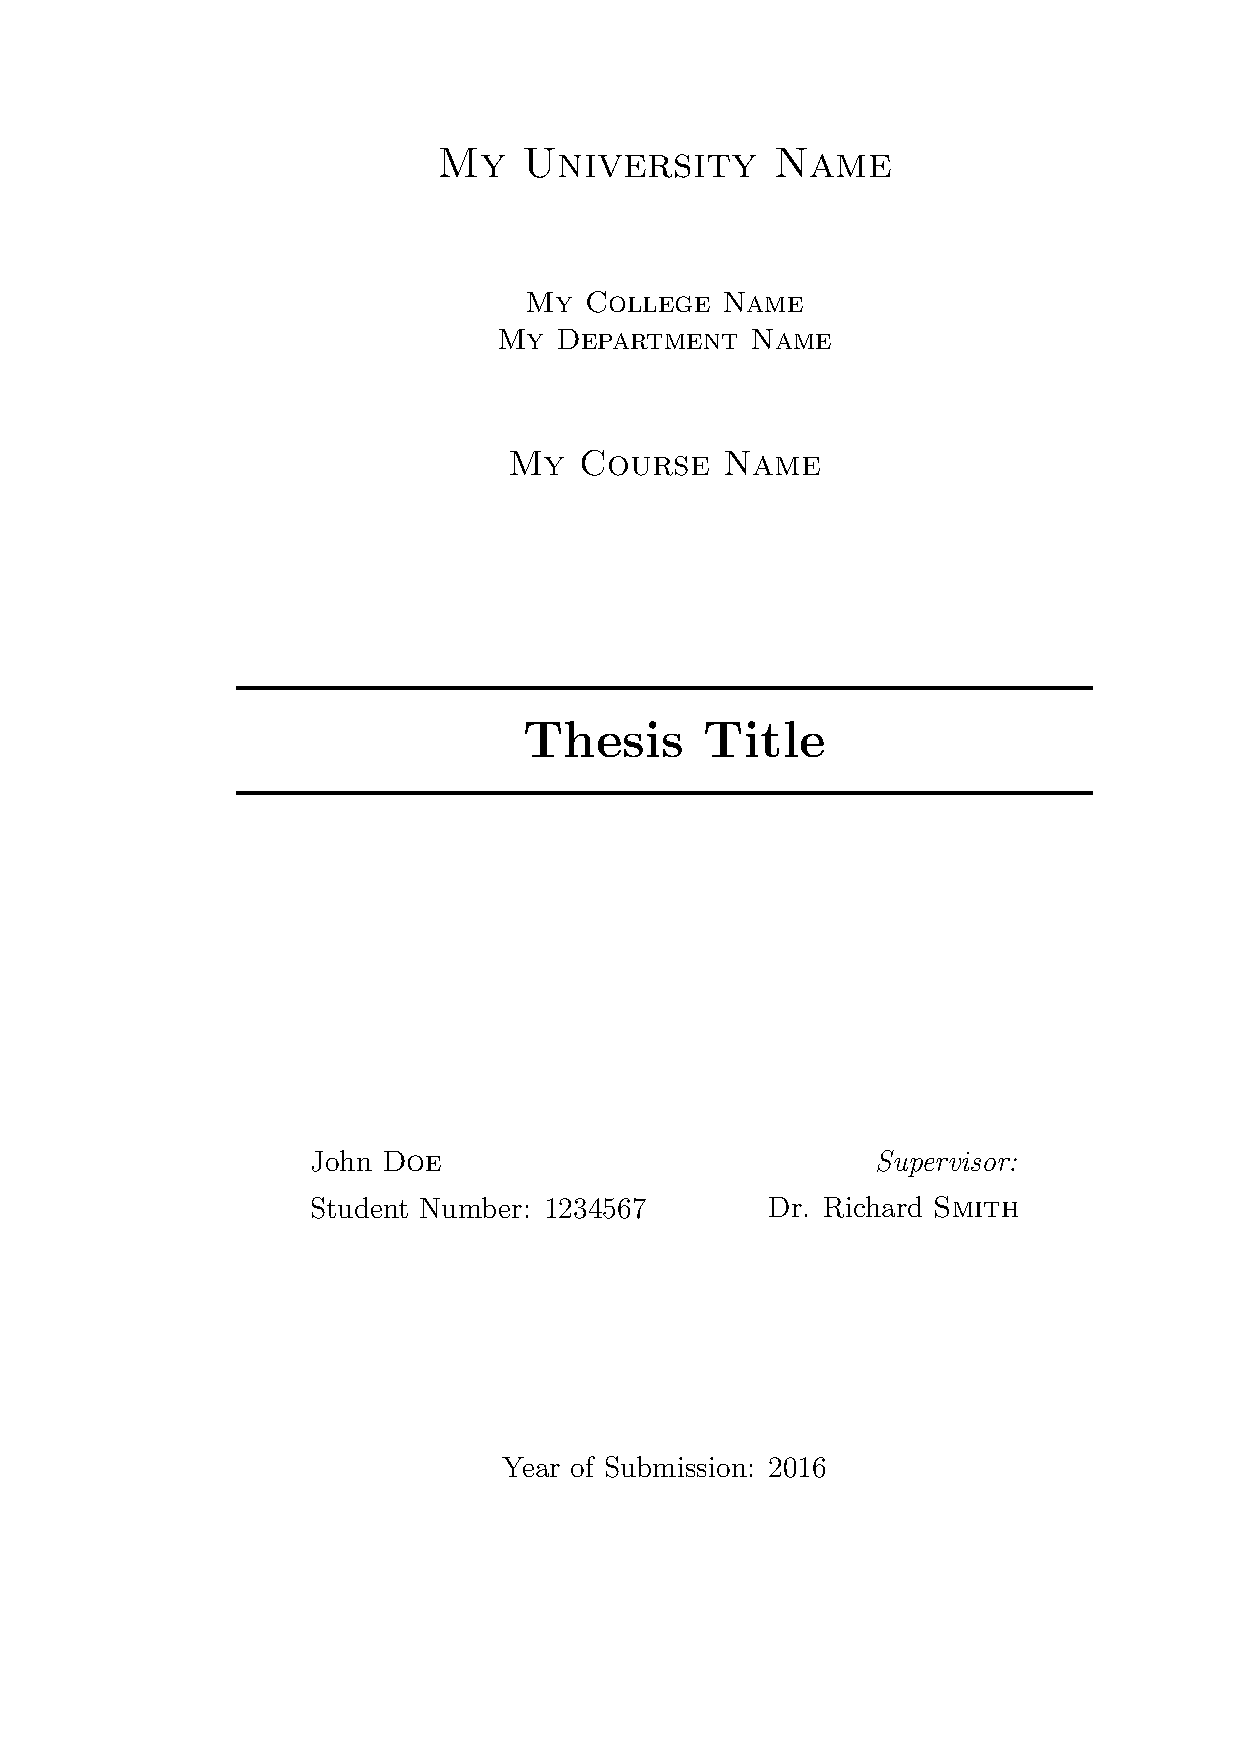
\includegraphics[width=.24\linewidth,page=1]{examples/fyp_example.pdf}
}
\fcolorbox{black}{white}{%
  \includegraphics[width=.24\linewidth,page=2]{examples/fyp_example.pdf}
}
\fcolorbox{black}{white}{%
  \includegraphics[width=.24\linewidth,page=3]{examples/fyp_example.pdf}
}
\fcolorbox{black}{white}{%
  \includegraphics[width=.24\linewidth,page=4]{examples/fyp_example.pdf}
}
\end{center}

\btVFill

\hfill\textsmaller{\LaTeX source available at \url{https://github.com/martinsbruveris/thesis-template}.} \\
\hfill\textsmaller{See also
\url{https://www.brunel.ac.uk/~mastmmb/mathwriting.html}.}

\medskip
\end{frame}

\begin{frame}
\frametitle{Highly Configurable Documents}
\framesubtitle{\texttt{memoir} and \textsmaller{KOMA}-Script Classes}

\begin{itemize}
\item Sectional headings
\item Running headers and footers
\item Good font, colour and illustration choices
\end{itemize}

%% See http://liantze.penguinattack.org/ebooks.html
\begin{center}
\onslide<2>{%
\fcolorbox{black}{white}{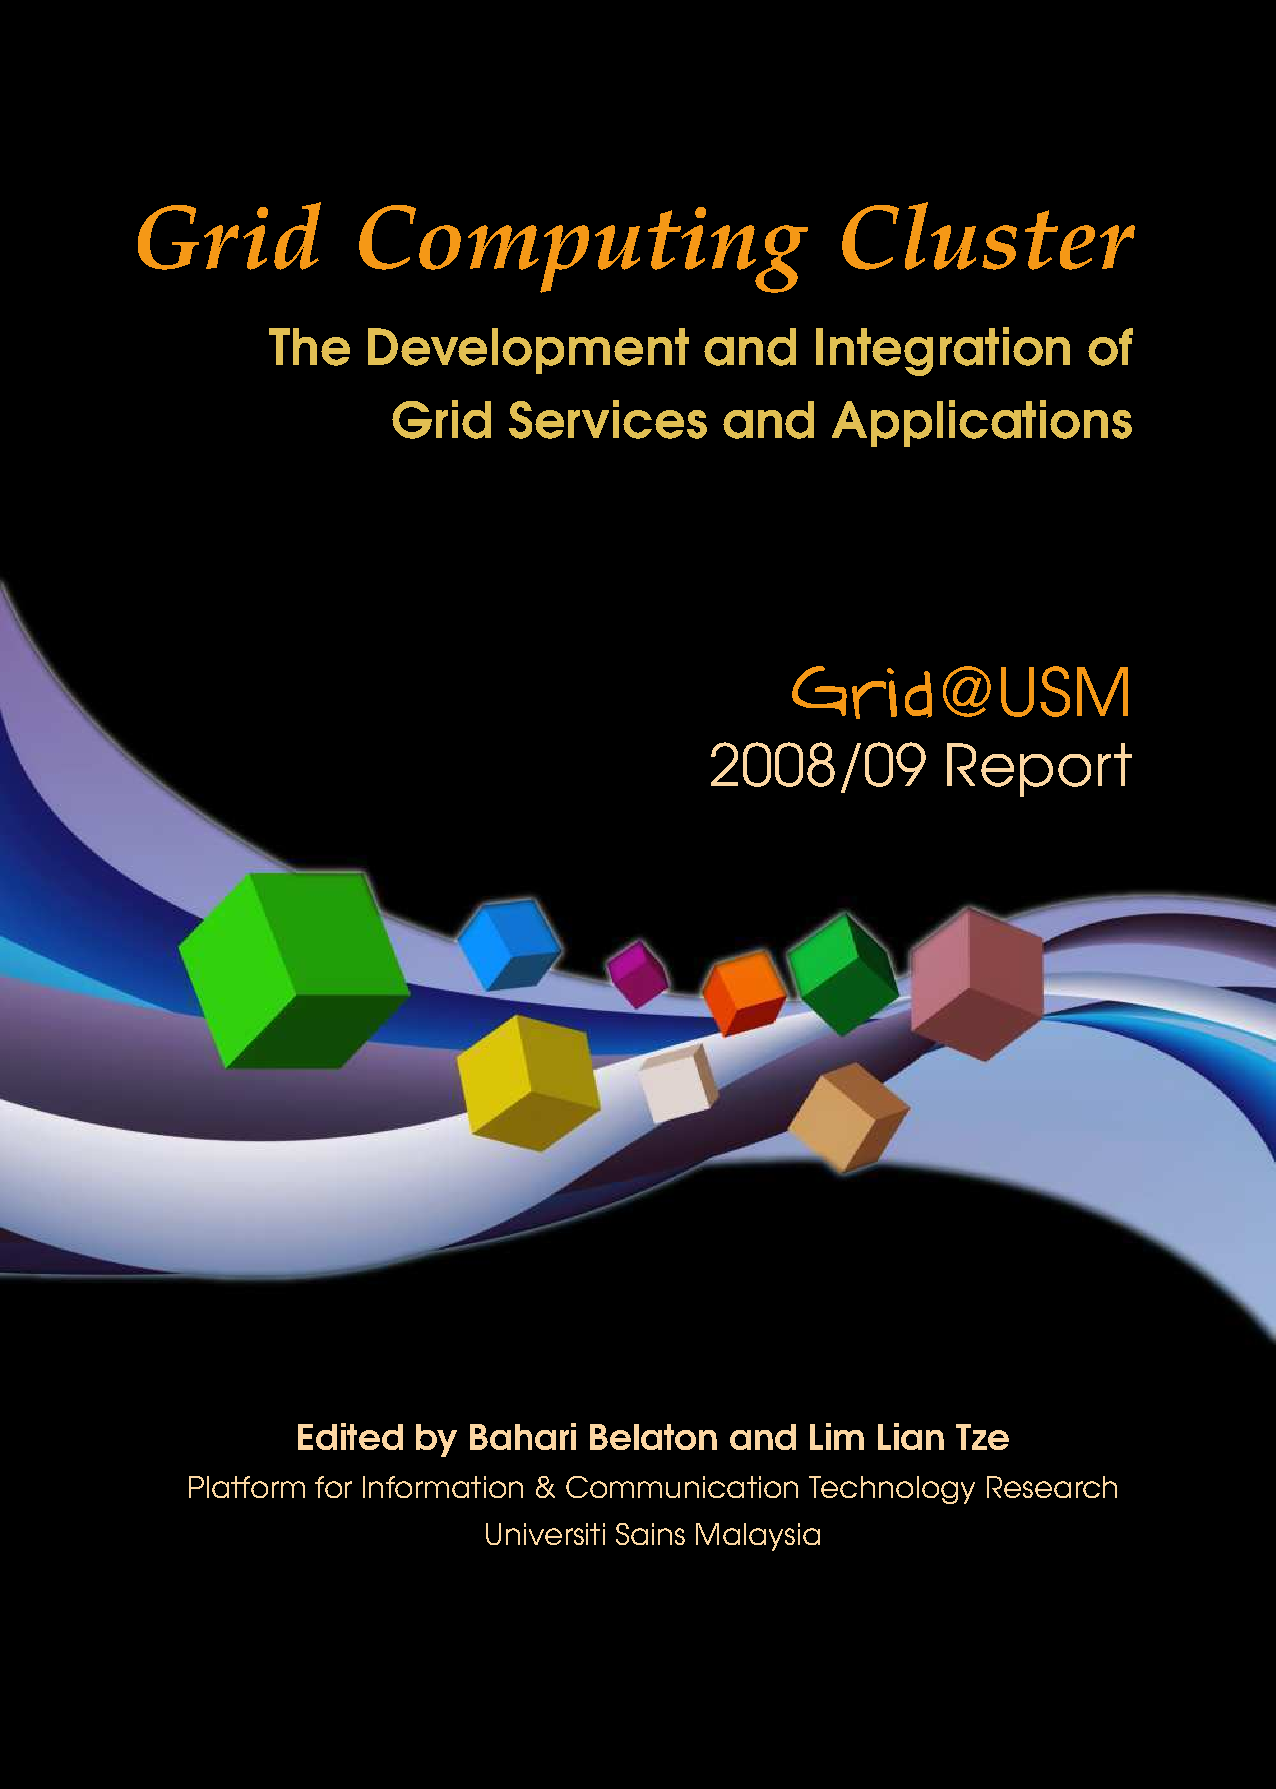
\includegraphics[width=.24\linewidth,page=1]{examples/GridBookExcerpt}}
\fcolorbox{black}{white}{\includegraphics[width=.24\linewidth,page=2]{examples/GridBookExcerpt}}
\fcolorbox{black}{white}{\includegraphics[width=.24\linewidth,page=3]{examples/GridBookExcerpt}}
\fcolorbox{black}{white}{\includegraphics[width=.24\linewidth,page=4]{examples/GridBookExcerpt}}
}
\end{center}
\end{frame}


\begin{frame}[fragile]
\frametitle{Presentation Slides}
\begin{itemize}
\item This presentation was made with \LaTeX.
\item<+-> Many possible classes: \texttt{powerdot}, \alert<2->{\texttt{beamer}}
\end{itemize}

\begin{columns}<+->
\begin{column}{.47\textwidth}
\begin{beamerboxesrounded}[width=\linewidth]{}
\vskip-1em
\begin{lstlisting}[basicstyle=\ttfamily\small,
moretexcs={usetheme,frametitle,frame,titleframe},
emph={beamer,frame},
escapechar={:},lineskip=-2pt]
\documentclass{beamer}
\usetheme{:\onslide<2>{\rlap{Warsaw\}}}%
\onslide<3|trans:0|handout:0>{\rlap{Szeged\}}}%
\onslide<4|trans:0|handout:0>{\rlap{Bergen\}}}%
\onslide<5|trans:0|handout:0>{\rlap{oxygen\}}}%
\onslide<6|trans:0|handout:0>{\rlap{Gelugor\}}}:

\author ...

\begin{document}
\titleframe

\section{Intro}

\begin{frame}
\frametitle{Some Background}
...
:\bfseries\color{Maroon}\textbackslash end:{frame}
\end{document}
\end{lstlisting}
\vspace*{-1em}
\end{beamerboxesrounded}
\end{column}
\begin{column}{.48\textwidth}
\centering
\onslide<2>{\fcolorbox{black}{white}{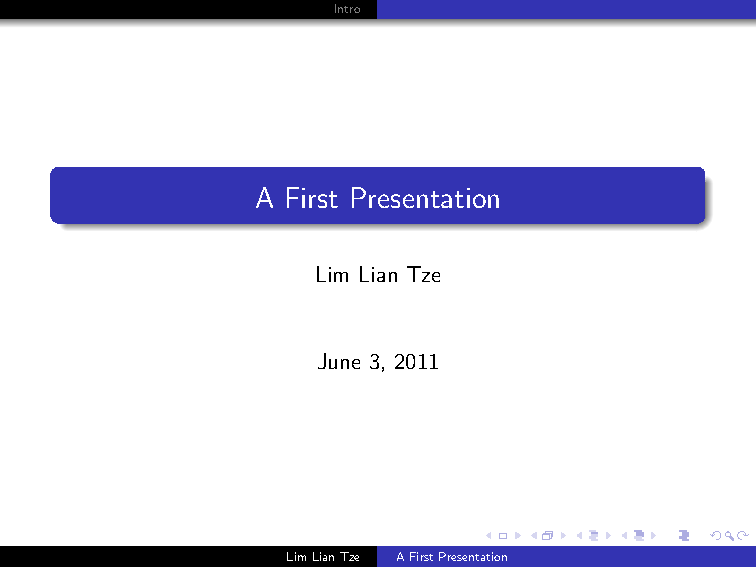
\includegraphics[width=.7\linewidth,page=1]{examples/beamer-Warsaw}}}%
\onslide<3|trans:0|handout:0>{\llap{\fcolorbox{black}{white}{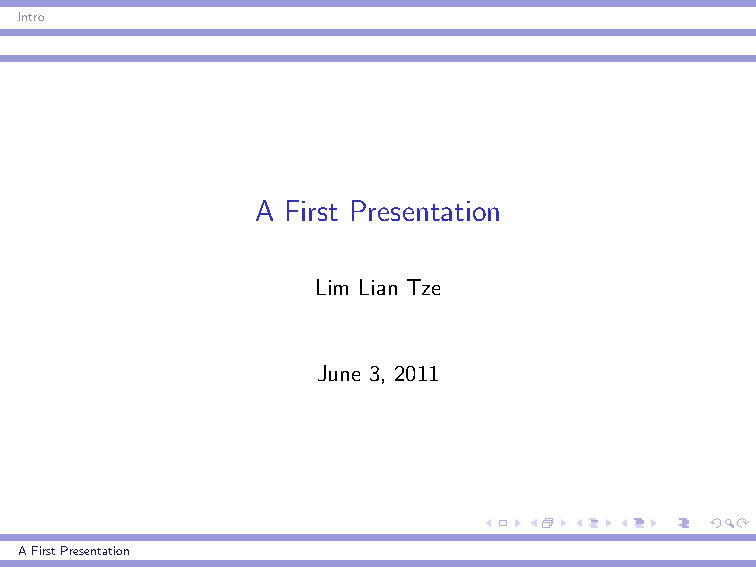
\includegraphics[width=.7\linewidth,page=1]{examples/beamer-Szeged}}
}}%
\onslide<4|trans:0|handout:0>{\llap{\fcolorbox{black}{white}{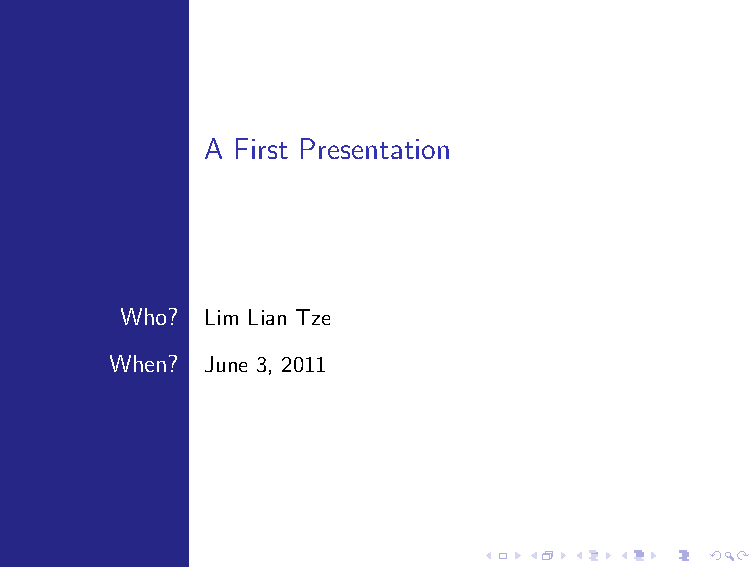
\includegraphics[width=.7\linewidth,page=1]{examples/beamer-Bergen}}
}}%
\onslide<5|trans:0|handout:0>{\llap{\fcolorbox{black}{white}{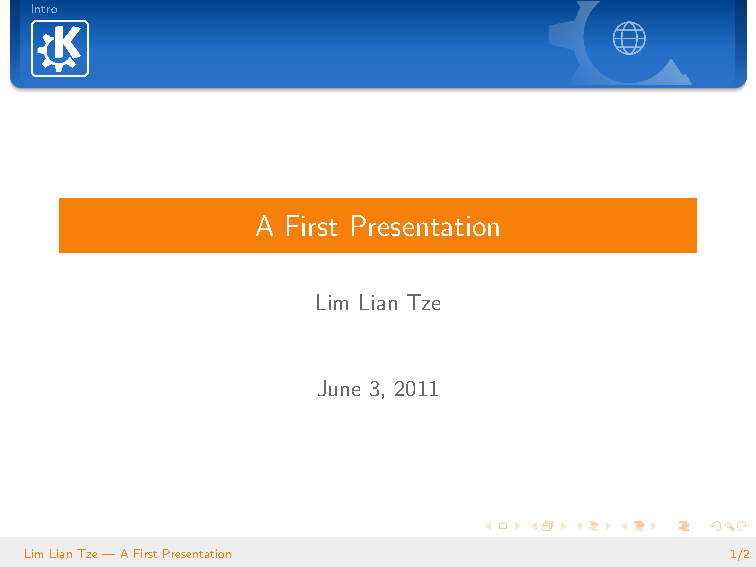
\includegraphics[width=.7\linewidth,page=1]{examples/beamer-Oxygen}}
}}%
\onslide<6|trans:0|handout:0>{\llap{\fcolorbox{black}{white}{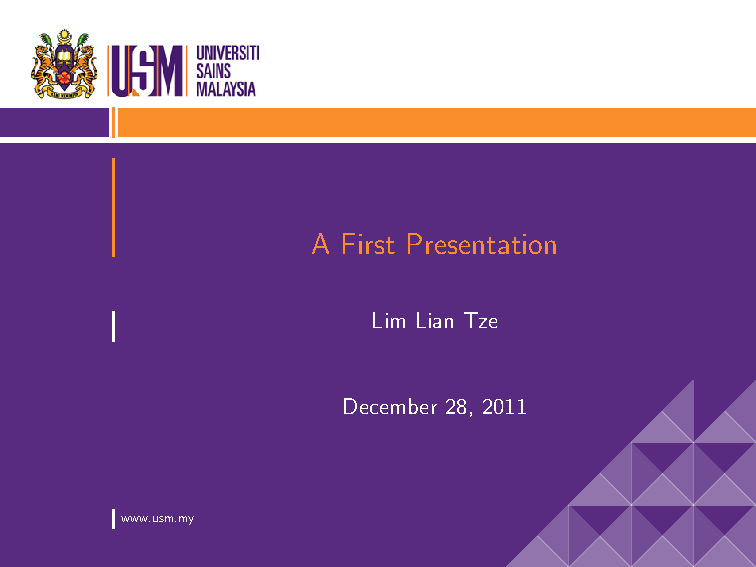
\includegraphics[width=.7\linewidth,page=1]{examples/beamer-Gelugor}}
}}
\onslide<2>{\fcolorbox{black}{white}{\includegraphics[width=.7\linewidth,page=2]{examples/beamer-Warsaw}}}%
\onslide<3|trans:0|handout:0>{\llap{\fcolorbox{black}{white}{\includegraphics[width=.7\linewidth,page=2]{examples/beamer-Szeged}}
}}%
\onslide<4|trans:0|handout:0>{\llap{\fcolorbox{black}{white}{\includegraphics[width=.7\linewidth,page=2]{examples/beamer-Bergen}}
}}%
\onslide<5|trans:0|handout:0>{\llap{\fcolorbox{black}{white}{\includegraphics[width=.7\linewidth,page=2]{examples/beamer-Oxygen}}
}}%
\onslide<6|trans:0|handout:0>{\llap{\fcolorbox{black}{white}{\includegraphics[width=.7\linewidth,page=2]{examples/beamer-Gelugor}}
}}
\end{column}
\end{columns}
\end{frame}

\begin{frame}[fragile]
\frametitle{Oversized Posters}
\begin{itemize}
\item Many possible solutions:\\\texttt{sciposter}, \texttt{flowfram}, \texttt{beamerposter}, \texttt{tikzposter}
\end{itemize}

% beamerposter
\begin{columns}
\begin{column}{.5\textwidth}
\begin{beamerboxesrounded}[width=\linewidth]{}
\begin{lstlisting}[basicstyle=\ttfamily\small,
moretexcs={usetheme,frametitle,frame},
emph={beamer,beamerposter,frame},
escapechar={:},lineskip=-2pt]
\documentclass{beamer}
\usepackage[orientation=portrait, size=a0]{beamerposter}
\usetheme{...}
\author ... % Meta-information

\begin{document}
\begin{frame}
... % Poster contents goes here
:\bfseries\color{Maroon}\textbackslash end:{frame}
\end{document}
\end{lstlisting}
\end{beamerboxesrounded}
\end{column}
\begin{column}{.48\textwidth}
\centering
% See http://latex-my.blogspot.com/2011/03/creating-academic-posters-and-printing.html
\fcolorbox{black}{white}{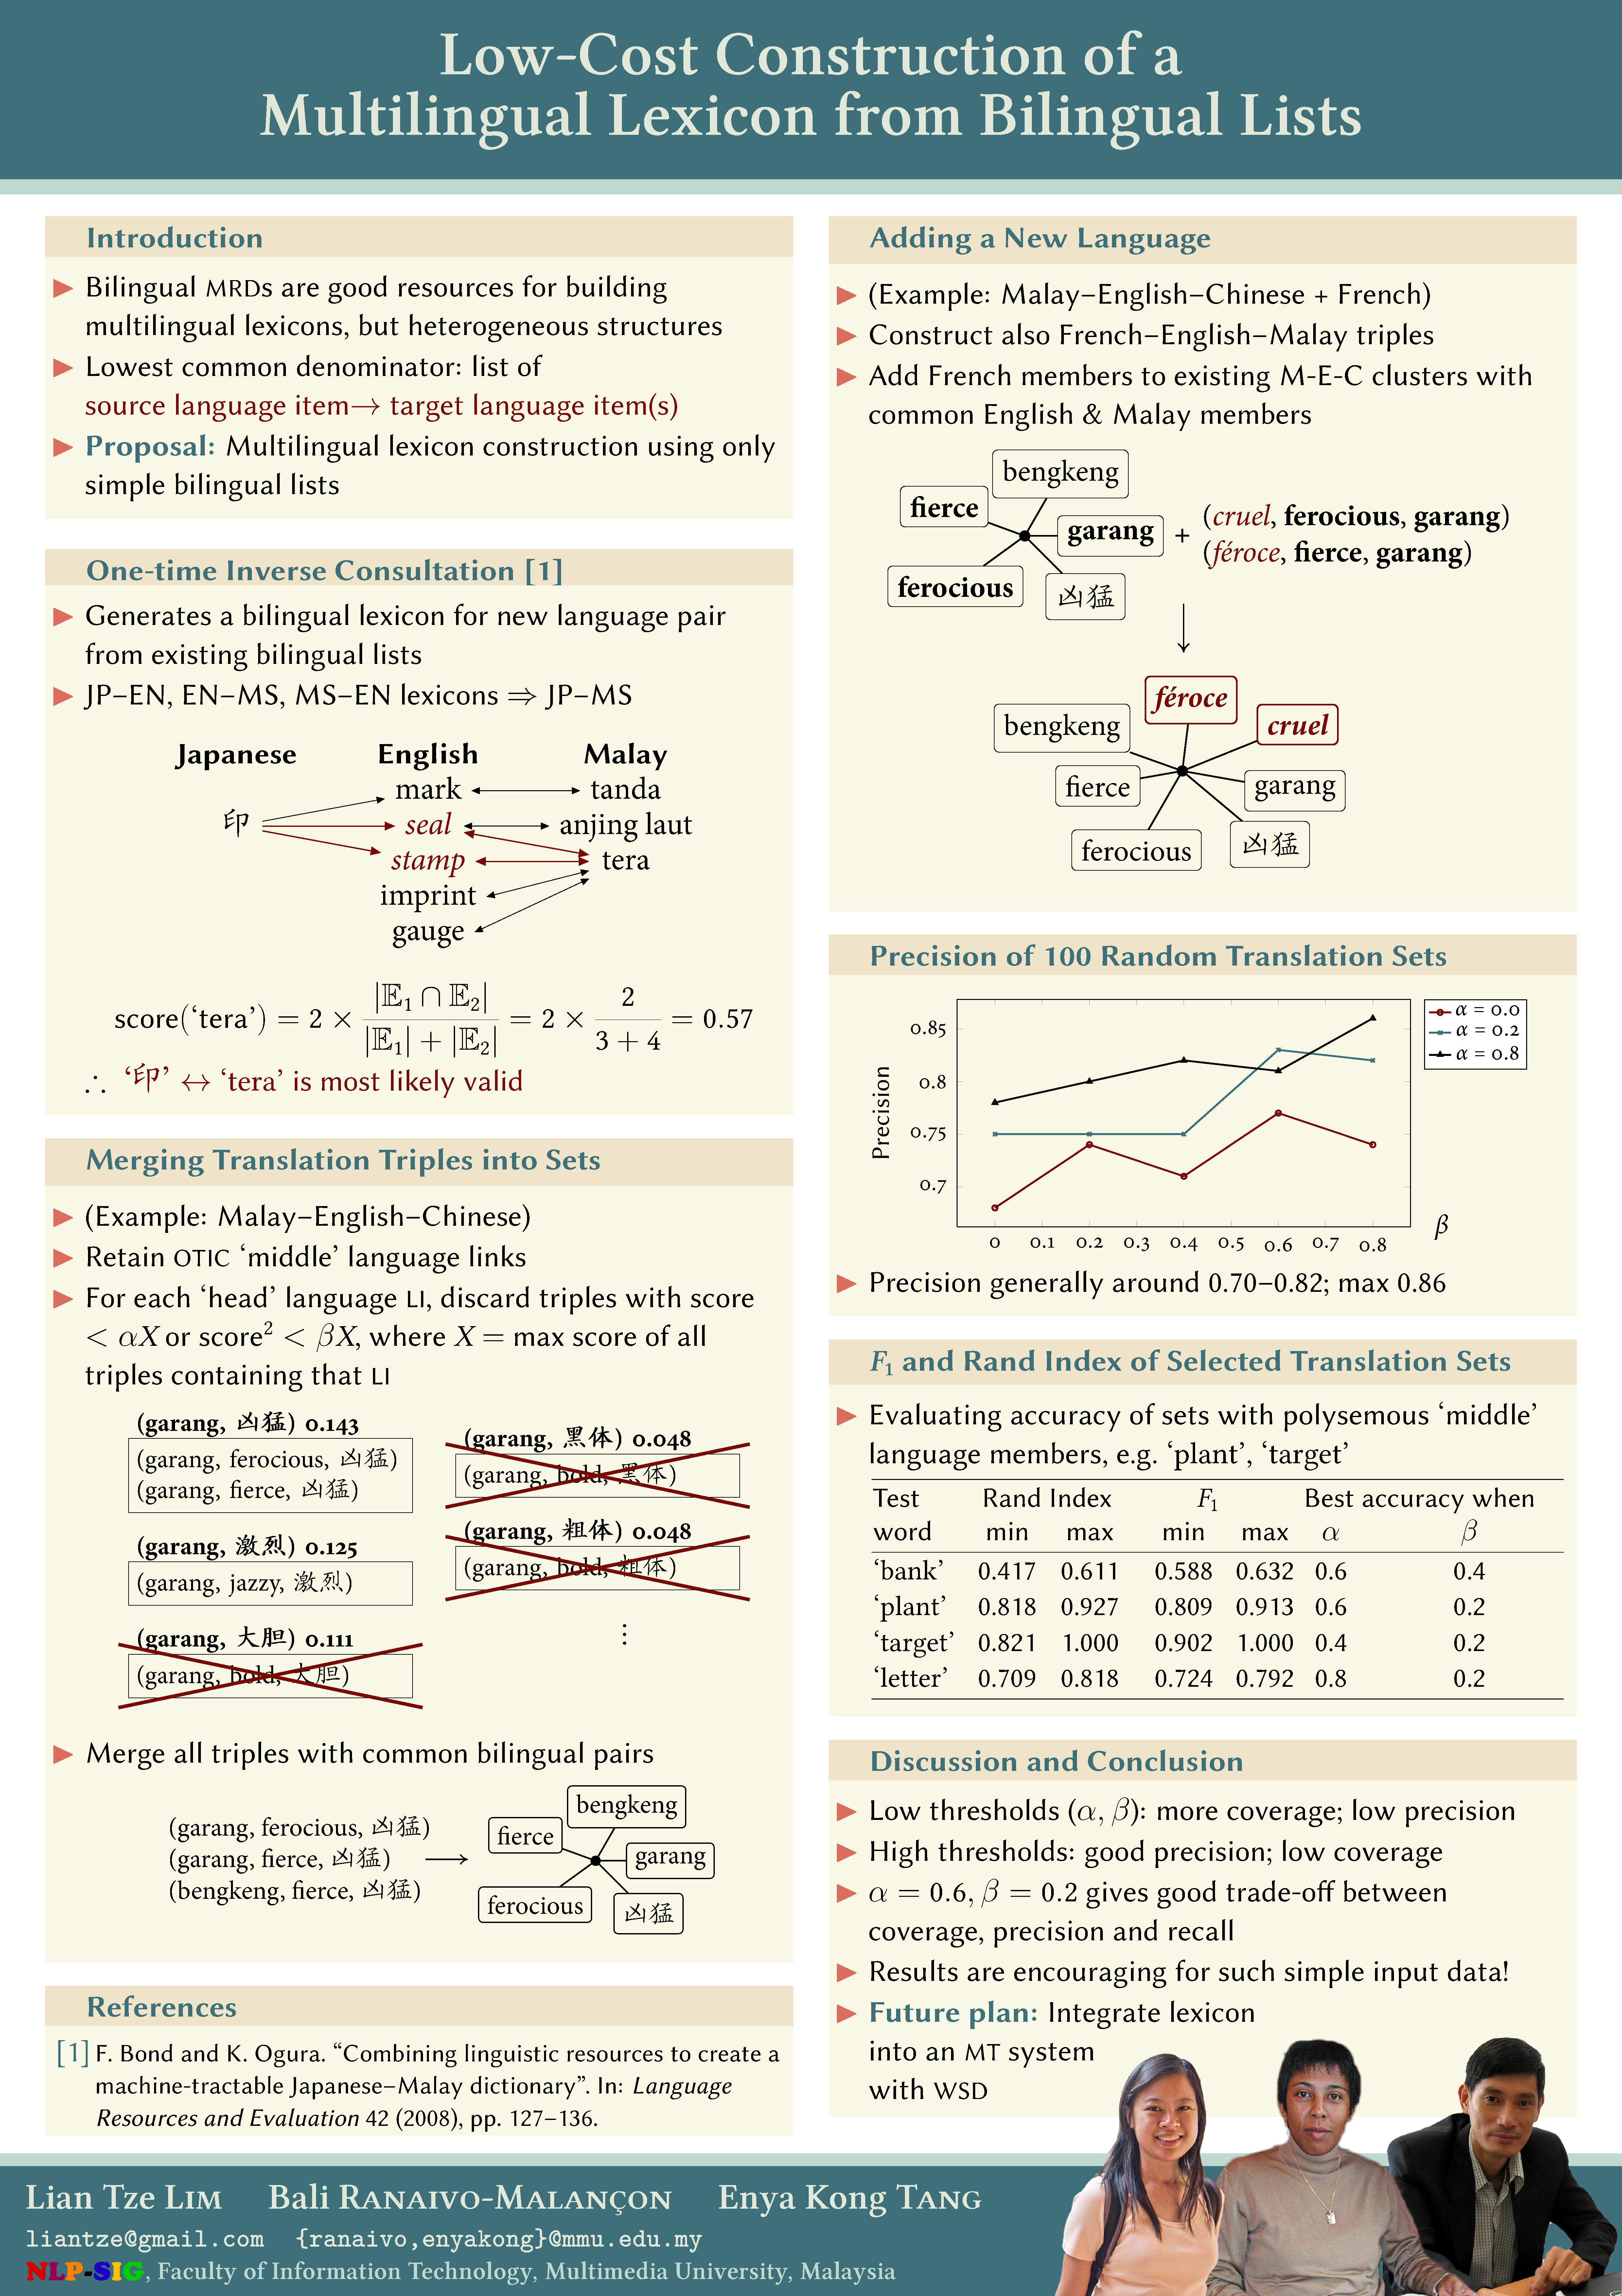
\includegraphics[width=.8\linewidth]{examples/cicling-poster-small.pdf}}
\end{column}
\end{columns}

\end{frame}

\begin{frame}[fragile]
\frametitle{Leaflets}

\texttt{leaflet} arranges contents into 6 pages on a foldable double-sided sheet.

\begin{columns}
\begin{column}{.496\textwidth}
\begin{beamerboxesrounded}[width=\linewidth]{}
\begin{lstlisting}[basicstyle=\ttfamily\small,lineskip=-2pt,emph={leaflet},moretexcs={maketitle}]
\documentclass[foldmark,a4paper]
{leaflet}
\author ... % Meta-information

\begin{document}
\maketitle
\section ...
... % Leaflet contents
\end{document}
\end{lstlisting}
\end{beamerboxesrounded}
\end{column}
\begin{column}{.48\textwidth}
\centering
% See http://latex-my.blogspot.com/2011/04/making-leaflets-with-l-t-e-x.html
\fcolorbox{black}{white}{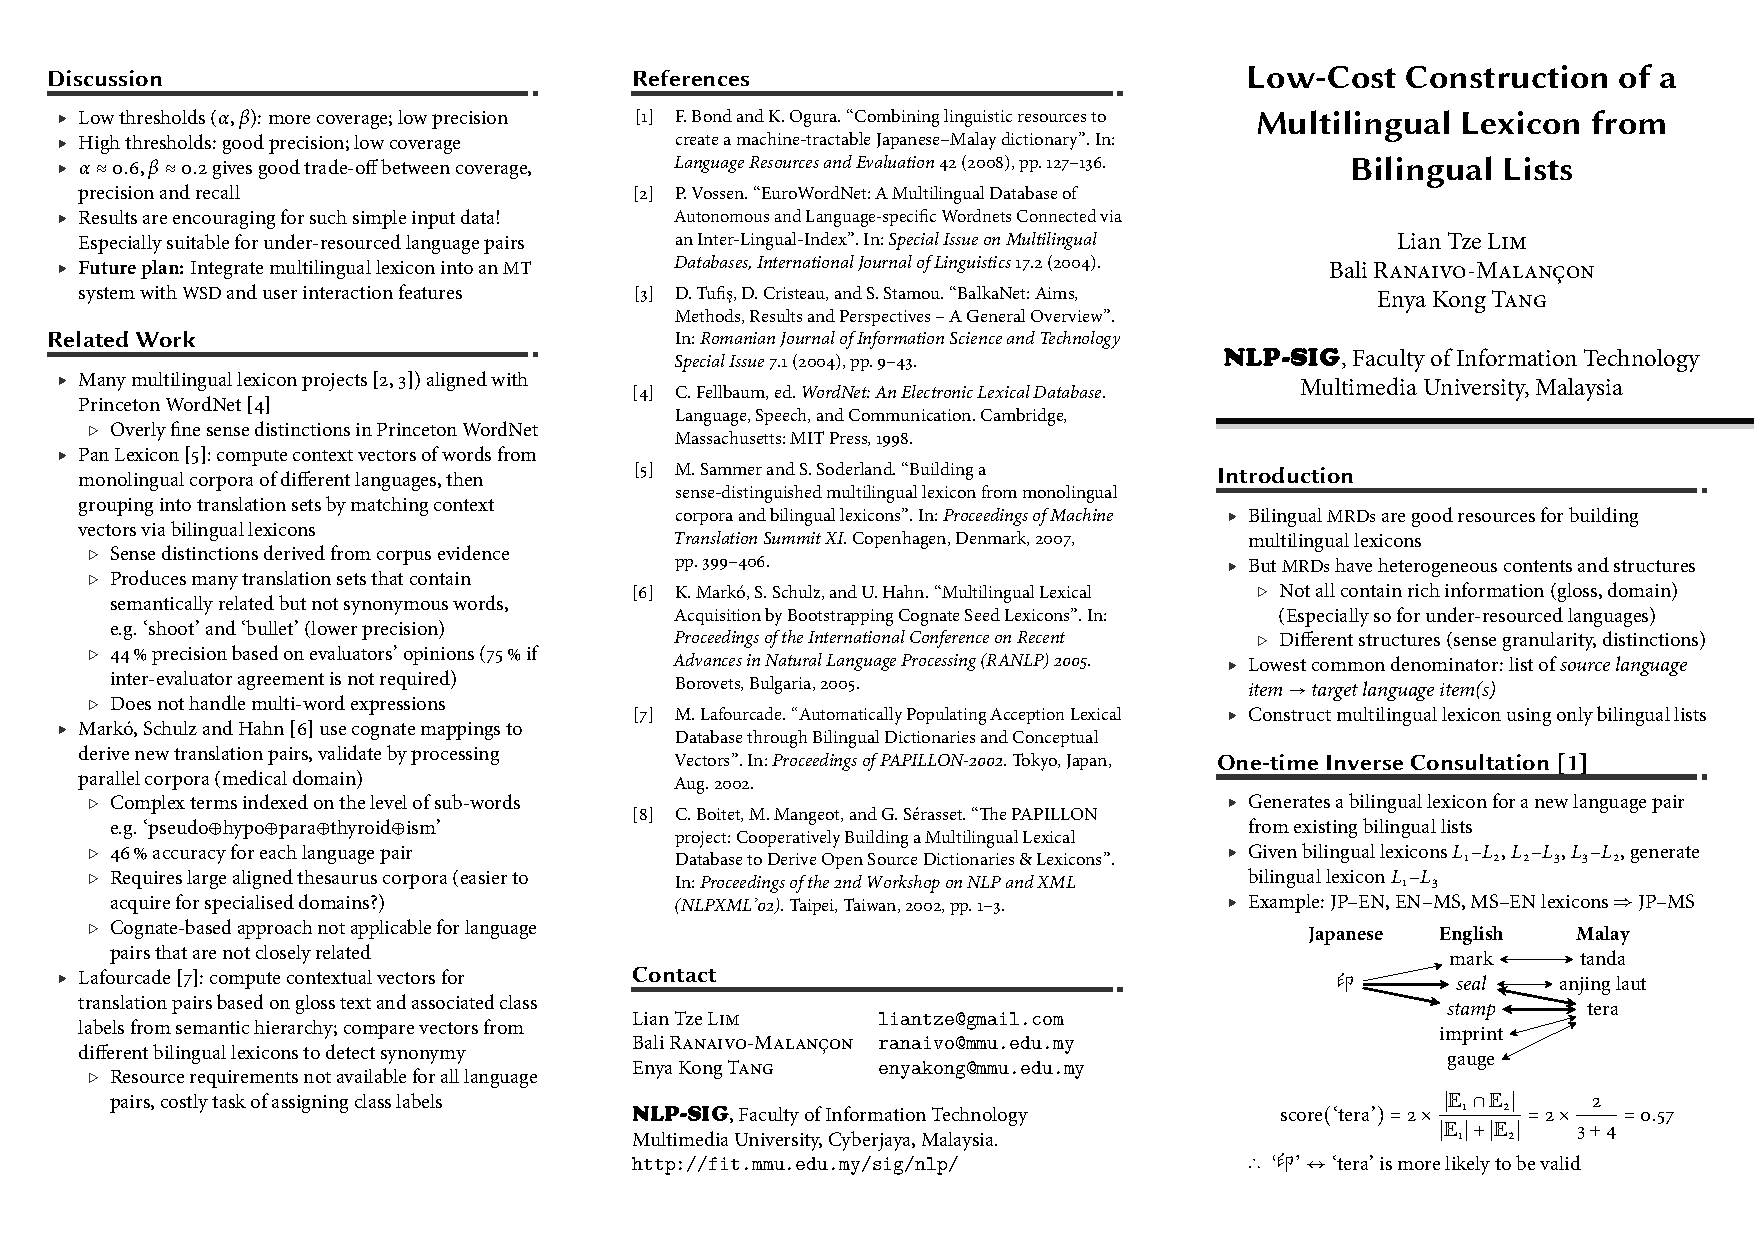
\includegraphics[width=.85\linewidth,page=1]{examples/cicling-handout.pdf}}
\fcolorbox{black}{white}{\includegraphics[width=.85\linewidth,page=2]{examples/cicling-handout.pdf}}\par
\end{column}
\end{columns}

\end{frame}


\begin{frame}[fragile]
\frametitle{Flash Cards}
\begin{columns}
\begin{column}{.47\textwidth}
\begin{beamerboxesrounded}{}
\vskip-1em
\begin{lstlisting}[basicstyle={\ttfamily\small},
emph={flashcards,flashcard},
moretexcs={cardfrontstyle,cardfrontfoot}]
\documentclass[avery5388,frame]
{flashcards}
\cardfrontstyle{headings}
\cardfrontfoot{Linux}

\begin{document}
\begin{flashcard}[Security]
{Certificate}
...
\end{flashcard}

\begin{flashcard}[Security]
{MAC ...}
...
\end{flashcard}
\end{document}
\end{lstlisting}
\vspace*{-1em}
\end{beamerboxesrounded}
\end{column}

\begin{column}{.53\textwidth}
\centering
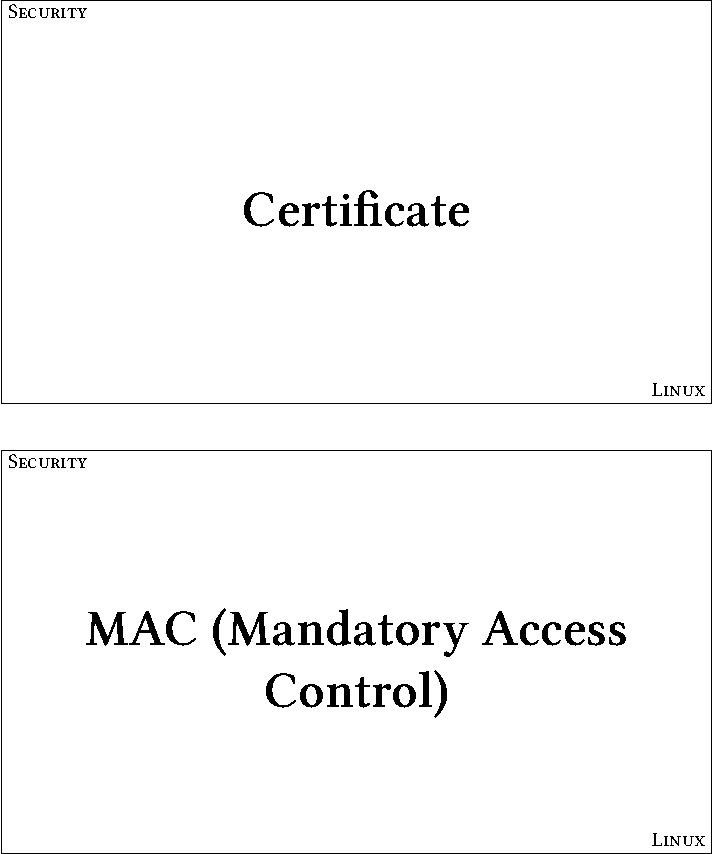
\includegraphics[width=.49\linewidth,page=1]{examples/flashcard-crop}\hfill
\includegraphics[width=.49\linewidth,page=2]{examples/flashcard-crop}
\par
\end{column}
\end{columns}
\end{frame}


%%% Local Variables:
%%% TeX-master: "talk"
%%% End:


% What kind of material can be typeset
% !TEX root=talk.tex
\section{Mathematics and Other Material}

%--------------------------------------------------------------------
%--- Mathematics
%--------------------------------------------------------------------

\begin{frame}[fragile]
\frametitle{Mathematics}
\begin{center}\begin{minipage}{.75\textwidth}\rmfamily
Equation \eqref{eq:gratio} relates the golden ratio and the Fibonacci series. 
Recall that the golden ratio is $\varphi = \frac{1}{2} (1 + \sqrt{5})$.

\begin{equation}\label{eq:gratio}
\varphi = 1 + \sum^{\infty}_{n=1}
                \frac{ (-1)^{n+1} }{ F_n F_{n+1} }
\end{equation}
\end{minipage}
\end{center}


\begin{center}\begin{minipage}{.9\textwidth}
\begin{beamerboxesrounded}{}
\vskip-1em
\begin{lstlisting}[escapechar=|,basicstyle=\ttfamily\small,moretexcs=eqref,emph={equation}]
Equation \eqref{eq:gratio} relates the golden ratio and the 
Fibonacci series. Recall that the golden ratio is |\textcolor{red}{\large\ttfamily\$}|\varphi =
\frac{1}{2} (1 + \sqrt{5})|\textcolor{red}{\large\ttfamily\$}|.

\begin{equation}\label{eq:gratio}
\varphi = 1 + \sum_{n=1}^{\infty}
                \frac{ (-1)^{n+1} }{ F_n F_{n+1} }
\end{equation}
\end{lstlisting}
\vspace*{-1em}
\end{beamerboxesrounded}
\end{minipage}
\end{center}

\end{frame}

%--------------------------------------------------------------------
%--- Program Listings
%--------------------------------------------------------------------

\begin{frame}[fragile]
\frametitle{Program Listings}

\begin{columns}
\begin{column}{.5\textwidth}
\begin{beamerboxesrounded}{}
\vspace{-1em}
\begin{lstlisting}[basicstyle=\ttfamily\footnotesize,escapechar=|,
emph={listings,lstlisting},moretexcs={color},commentstyle={},]
\usepackage{listings,xcolor}
...
\begin{lstlisting}[language=matlab,
basicstyle=\ttfamily,
keywordstyle=\bfseries\color{red},
commentstyle=\sffamily\color{green},
stringstyle=\rmfamily\color{orange}]
disp('Hello World');

% Calculate golden ratio
F = zeros(10, 1);
F(1:2) = [1, 1];
phi = 1; % Initial value  

for j=1:8
    F(j+2) = F(j+1) + F(j);
    phi = phi + (-1)^(j+1) ...
            / (F(j+1) * F(j));
end
|\bfseries\color{Maroon}\textbackslash end|{lstlisting}
\end{lstlisting}
\vspace{-1em}
\end{beamerboxesrounded}
\end{column}
\hfill\begin{column}{.5\textwidth}
\begin{lstlisting}[language=matlab,escapechar=~,lineskip=-2pt,
basicstyle=\ttfamily,
commentstyle=\upshape\sffamily\small\color{SeaGreen4},keepspaces=true,
keywordstyle=\bfseries\color{Maroon},stringstyle=\rmfamily\color{Sienna2}]
disp('Hello World');

% Calculate golden ratio
F = zeros(10, 1);
F(1:2) = [1, 1];
phi = 1; % Initial value

for j=1:8
    F(j+2) = F(j+1) + F(j);
    phi = phi + (-1)^(j+1) ...
            / (F(j+1) * F(j));
end
\end{lstlisting}
\end{column}
\end{columns}
\end{frame}

%--------------------------------------------------------------------
%--- Graphs and Diagrams
%--------------------------------------------------------------------

\begin{frame}[fragile]
\frametitle{Graphs and Diagrams}

\begin{columns}
\begin{column}{.65\textwidth}
\begin{beamerboxesrounded}{}
\vspace{-1em}
\begin{lstlisting}[basicstyle=\ttfamily,escapechar=|,
emph={xy,xymatrix},moretexcs={color},commentstyle={},]
\usepackage[all]{xy}

\[
  \xymatrix{
    A \ar[r]^f \ar[dr]_{f \circ g} &
    B \ar[d]^g \ar[dr]^{g \circ h} \\
    & C \ar[r]_h & D
  }
\]
\end{lstlisting}
\vspace{-1em}
\end{beamerboxesrounded}
\end{column}
\hfill\begin{column}{.35\textwidth}
{\Large
\[
\xymatrix{
A \ar[r]^f \ar[dr]_{f \circ g}
& B \ar[d]^g \ar[dr]^{g \circ h} \\
& C \ar[r]_h & D
 }
\]
}
\end{column}
\end{columns}
\end{frame}

%--------------------------------------------------------------------
%--- Tables
%--------------------------------------------------------------------

\begin{frame}[fragile]
\frametitle{Tables}
\begin{center}\rmfamily
\begin{tabular}{lrrr} \toprule
Year ending Mar 31 & 2016 & 2015 & 2014 \\ \midrule
Revenue & 14580.20 & 11900.40 & 8290.30 \\
Cost of sales & 6740.20 & 5650.10 & 4524.20 \\ \cmidrule(r){2-4}
\emph{Gross profit} & 7840.00 & 6250.30 & 3766.10 \\ 
\bottomrule
\end{tabular}
\end{center}

\begin{beamerboxesrounded}{}
\vskip-1em
\begin{lstlisting}[basicstyle=\ttfamily\small,
moretexcs={toprule,midrule,cmidrule,bottomrule,lightrulewidth},
alsoletter={23->}, emph={tabular,booktabs},
emph={[2]{b2-b3,>}}]
\usepackage{booktabs}
...
\begin{tabular}{lrrr} \toprule
  Year ending Mar 31 & 2016 & 2015 & 2014 \\ \midrule
  Revenue & 14580.20 & 11900.40 & 8290.30 \\
  Cost of sales & 6740.20 & 5650.10 & 4524.20 \\ \cmidrule(r){2-4}
  \emph{Gross profit} & 7840.00 & 6250.30 & 3766.10 \\ \bottomrule
\end{tabular}
\end{lstlisting}
\vspace{-1em}
\end{beamerboxesrounded}

\end{frame}

%--------------------------------------------------------------------
%--- Graph Plots
%--------------------------------------------------------------------

\begin{frame}[fragile]
\frametitle{Graph Plots}

\begin{columns}[totalwidth=\textwidth]
\begin{column}{0.6\textwidth}

% %\pgfplotsset{height=.75\textheight,width=\linewidth}
\begin{tikzpicture}[transform shape]
\begin{loglogaxis}[xlabel=DoF,
       width=\textwidth,
       height=0.6\textwidth]
\addplot table[x=dof,y=La] {examples/datafile.dat}; \addlegendentry{$L_\alpha$};
\addplot table[x=dof,y=Lb] {examples/datafile.dat}; \addlegendentry{$L_\beta$};
\end{loglogaxis} 
\end{tikzpicture}

\end{column}
\begin{column}{0.4\textwidth}

Contents of \texttt{datafile.dat}
\begin{beamerboxesrounded}{}
\vspace{-1em}
\lstinputlisting{examples/datafile.dat}
\vspace{-1em}
\end{beamerboxesrounded}

\end{column}
\end{columns}

%\medskip

\begin{beamerboxesrounded}{}
\vskip-1em
\begin{lstlisting}[basicstyle=\ttfamily\footnotesize,
emph={pgfplots,tikzpicture,loglogaxis},
moretexcs={addplot, table, addlegendentry,text},lineskip=-2pt]
\usepackage{pgfplots}
...
\begin{tikzpicture}
\begin{loglogaxis}[xlabel=DoF]
\addplot table[x=dof,y=La]{datafile.dat}; \addlegendentry{$L_\alpha$};
\addplot table[x=dof,y=Lb]{datafile.dat};  \addlegendentry{$L_\beta$};
\end{loglogaxis} 
\end{tikzpicture} 
\end{lstlisting}
\vspace{-1em}
\end{beamerboxesrounded}

\end{frame}

%--------------------------------------------------------------------
%--- Gantt Charts
%--------------------------------------------------------------------

\begin{frame}[fragile]
\frametitle{Gantt Charts}

\scalebox{.85}{\rmfamily
\begin{ganttchart}%
[y unit title=0.4cm,
y unit chart=0.5cm,
vgrid=true,
title/.style={draw=none, fill=RoyalBlue!50!black},
title label font=\sffamily\bfseries\color{white}, title label anchor/.style={below=-1.6ex},
title left shift=.05,
title right shift=-.05,
title height=1,
bar/.style={draw=none, fill=OliveGreen!75},
bar height=.6,
bar label font=\normalsize\color{black!50},
group right shift=0,
group top shift=.6,
group height=.3, group peaks height=.2,
bar incomplete/.style={fill=Maroon}]{1}{16} 
\gantttitle{2016}{4} \gantttitle{2017}{12} \\ 
\ganttbar%
[progress=100, bar progress label font=\small\color{OliveGreen!75}, progress label anchor/.style={right=4pt},
bar label font=\normalsize\color{OliveGreen},
name=pp]%
  {Preliminary Project}{1}{4} \\
\ganttset{progress label text={}, link/.style={black, -to}}
\ganttgroup{Objective 1}{5}{16} \\
\ganttbar[progress=50, name=T1A]{Task A}{5}{10} \\
\ganttlinkedbar[progress=0]{Task B}{11}{16} \\
\ganttgroup{Objective 2}{5}{16} \\
\ganttbar[progress=75, name=T2A]{Task A}{5}{13} \\
\ganttlinkedbar[progress=0]{Task B}{14}{16}
\end{ganttchart}
}

\begin{beamerboxesrounded}{}
\vskip-1em
\begin{lstlisting}[basicstyle=\ttfamily\footnotesize,lineskip=-2pt,
moretexcs={gantttitle,ganttbar,ganttlink,ganttgroup,ganttlinkedbar},
emph={pgfgantt,tikzpicture,ganttchart}]
\usepackage{pgfgantt}
...
\begin{ganttchart}[...settings...]{1}{16} 
\gantttitle{2016}{4} \gantttitle{2017}{12} \\ 
\ganttbar[progress=100]{Preliminary Project}{1}{4} \\ 
\ganttgroup{Objective 1}{5}{16} \\ 
\ganttbar[progress=50, name=T1A]{Task A}{5}{10} \\ 
\ganttlinkedbar[progress=0]{Task B}{11}{16} \\ 
...
\end{ganttchart} 
\end{lstlisting}
\vspace{-1em}
\end{beamerboxesrounded}

\end{frame}

%--------------------------------------------------------------------
%--- Chemistry
%--------------------------------------------------------------------

\begin{frame}[fragile]
\frametitle{Chemical Equations and Molecules}

\begin{center}\rmfamily\small
\ce{Zn^2+ <=>[\ce{+ 2OH-}][\ce{+ 2H+}]
$\underset{\text{amphoteres Hydroxid}}{\ce{Zn(OH)2 v}}$
<=>C[+2OH-][{+ 2H+}]
$\underset{\text{Hydroxozikat}}{\cf{[Zn(OH)4]^2-}}$
}
\hfil
\chemfig{H-C(-[2]H)(-[6]H)-C(-[7]H)=[1]O}
\end{center}

\begin{beamerboxesrounded}{}
\vskip-1em
\begin{lstlisting}[basicstyle=\ttfamily\small,moretexcs={ce,chemfig,underset,text,cf},
emph={mhchem,chemfig}]
\usepackage[version=3]{mhchem}   % sufficient for chemical equations
\usepackage{chemfig}             % for 2-D molecule drawings
...
\ce{Zn^2+ <=>[\ce{+ 2OH-}][\ce{+ 2H+}]
$\underset{\text{amphoteres Hydroxid}}{\ce{Zn(OH)2 v}}$
<=> C[+2OH-][{+ 2H+}] 
$\underset{\text{Hydroxozikat}}{\cf{[Zn(OH)4]^2-}}$ }

\chemfig{H-C(-[2]H)(-[6]H)-C(-[7]H)=[1]O}
\end{lstlisting}
\vspace*{-1em}
\end{beamerboxesrounded}

\end{frame}

%--------------------------------------------------------------------
%--- Circuits and SI Units
%--------------------------------------------------------------------

\begin{frame}[fragile]
\frametitle{Circuits and SI Units}
\begin{columns}
\begin{column}{.49\textwidth}\rmfamily
\begin{circuitikz}[transform shape,scale=.9]
\draw (0,0) node[anchor=east] {B}  to[short, o-*] (1,0)    to[R=20<\ohm>, *-*] (1,2)
  to[R=10<\ohm>, v=$v_x$] (3,2) -- (4,2)
  to[ cI=$\frac{\si{\siemens}}{5} v_x$, *-*] (4,0) -- (3,0)  to[R=5<\ohm>, *-*] (3,2)
  (3,0) -- (1,0)   (1,2) to[short, -o] (0,2) node[anchor=east]{A}
;\end{circuitikz}
\end{column}
\begin{column}{.49\textwidth}
\begin{itemize}\rmfamily
\item \SI{3.45d4}{\square\volt\cubic\lumen\per\farad}
\item \SIlist[per-mode=symbol]{40;85;103}{\kilo\metre\per\hour}
\end{itemize}
\end{column}
\end{columns}

\medskip

\begin{beamerboxesrounded}{}
\vskip-1em
\begin{lstlisting}[basicstyle=\ttfamily\footnotesize,lineskip=-2pt,
moretexcs={draw,si,siemens,ohm,SI,SIlist,square,volt,cubic,lumen,per,farad,kilo,metre,hour},
emph={siunitx,circuitikz},emph={[2]{draw,node,to}}
]
\usepackage{siunitx}
\usepackage[siunitx]{circuitikz}
...
\begin{circuitikz}
\draw (0,0) node[anchor=east] {B}
  to[short, o-*] (1,0)    to[R=20<\ohm>, *-*] (1,2)
  to[R=10<\ohm>, v=$v_x$] (3,2) -- (4,2)
  to[ cI=$\frac{\si{\siemens}}{5} v_x$, *-*] (4,0) -- (3,0)
  to[R=5<\ohm>, *-*] (3,2)
  (3,0) -- (1,0)   (1,2) to[short, -o] (0,2) node[anchor=east]{A}
;\end{circuitikz}

\SI{3.45d4}{\square\volt\cubic\lumen\per\farad}
\SIlist[per-mode=symbol]{40;85;103}{\kilo\metre\per\hour}
\end{lstlisting}
\vspace{-1em}
\end{beamerboxesrounded}
\end{frame}


\begin{frame}[fragile]
\frametitle{Bar Codes}
%%% CAUTION!!! This takes a LOOONG time to compile if you're using pdflatex. I'm just going to load the already generated PDFs instead.

% \begin{pspicture}
% \psbarcode{MECARD:N:Malaysia Open Source Conference 2011;TEL:+60196085482;URL:http://www.mosc.my/;EMAIL:secretariat@mosc.my;ADR:Bayview Beach Resort, Baru Ferringgi Penang;NOTE:Malaysia Open Source Conference 2011 (MOSC2011);;}{eclevel=L width=0.75 height=0.75}{qrcode}
% \end{pspicture}\;

\includegraphics[page=1]{images/talk-pics}\;
% \begin{pspicture}
% \psbarcode[scalex=0.7,scaley=0.7]{9781860742712}{ includetext guardwhitespace }{ean13} 
% \end{pspicture}\;

\includegraphics[page=2]{images/talk-pics}\;
% \begin{pspicture}
% \psbarcode[scalex=0.7,scaley=0.7]{978-3-86541-114}{includetext guardwhitespace}{isbn} 
% \end{pspicture}\;\;

\includegraphics[page=3]{images/talk-pics}\;
% \begin{pspicture}
% \psbarcode[scalex=0.7,scaley=0.7]{^453^178^121^239}{ columns=2 rows=10}{pdf417}
% \end{pspicture}%

\includegraphics[page=4]{images/talk-pics}
\llap{\raisebox{0.45in}{
\includegraphics[page=5]{images/talk-pics}%
% \begin{pspicture}
% \psbarcode[scalex=0.6,scaley=0.6]{LE28HS9Z}{includetext}{royalmail}
% \end{pspicture}
}}

\bigskip

\begin{beamerboxesrounded}{}
\vskip-1em
\begin{lstlisting}[moretexcs={psbarcode},escapechar=|,basicstyle=\ttfamily\footnotesize,
emph={pst-barcode},emph={[2]{qrcode,ean13,isbn,pdf417,royalmail,}},
alsoletter={1347-}
]
\usepackage{auto-pst-pdf}  % Needed if running pdflatex; must use option -shell-escape
\usepackage{pstricks,pst-barcode}
...
|\color{Maroon}\bfseries\textbackslash begin|{pspicture}
\psbarcode{MECARD:N:Malaysia Open Source Conference...}{eclevel=L}{qrcode}
\psbarcode{9781860742712}{includetext guardwhitespace}{ean13} 
\psbarcode{978-3-86541-114}{includetext guardwhitespace}{isbn} 
\psbarcode{LE28HS9Z}{includetext}{royalmail}
\psbarcode{^453^178^121^239}{columns=2 rows=10}{pdf417}
|\color{Maroon}\bfseries\textbackslash end|{pspicture} 
\end{lstlisting}
\vspace{-1em}
\end{beamerboxesrounded}
\end{frame}

%--------------------------------------------------------------------
%--- Smart Diagrams
%--------------------------------------------------------------------

\begin{frame}[fragile]
\frametitle{`Smart Diagrams'}
\begin{columns}[T]

\begin{column}{.49\textwidth}
\resizebox{\linewidth}{!}{\smartdiagram[bubble diagram]{Planning Cycle,Assess,Plan,Implement,Renew}}

\begin{beamerboxesrounded}{}
\vskip-1em
\begin{lstlisting}[basicstyle=\ttfamily\footnotesize,lineskip=-2pt]
\usepackage{smartdiagram}
\smartdiagram[bubble diagram]{
  Planning Cycle,Assess,Plan,
  Implement,Renew}
\end{lstlisting}
\vspace{-1em}
\end{beamerboxesrounded}
\end{column}

\begin{column}{.49\textwidth}
\resizebox{\linewidth}{!}{\smartdiagram[priority descriptive diagram]{Assess,Plan,Implement,Renew}}

\begin{beamerboxesrounded}{}
\vskip-1em
\begin{lstlisting}[basicstyle=\ttfamily\footnotesize,lineskip=-2pt]
\usepackage{smartdiagram}
\smartdiagram
  [priority descriptive diagram]{
  Assess,Plan,Implement,Renew}
\end{lstlisting}
\vspace{-1em}
\end{beamerboxesrounded}
\end{column}

\end{columns}

% \resizebox{\linewidth}{\smartdiagram[priority descriptive diagram]{Planning Cycle,Assess,Plan,Implement,Renew}}
\end{frame}

%--------------------------------------------------------------------
%--- Crossword Puzzles
%--------------------------------------------------------------------

\begin{frame}[fragile]
\frametitle{Crossword Puzzles}
\begin{columns}
\begin{column}{.3\textwidth}\rmfamily
\begin{Puzzle}{5}{3}
|* |* |[1]E|X |* |.
|[2]A|[3]S|T |* |[4]T|.
|* |[5]P|A |R |T |.
\end{Puzzle}
\end{column}
\begin{column}{.65\textwidth}\rmfamily
\begin{PuzzleClues}{
\textbf{Across:} }
  \Clue{1}{EX}{unit of measure}
  \Clue{2}{AST}{\(\ast\)}
  \Clue{5}{PART}{sectioning unit}
\end{PuzzleClues}
\begin{PuzzleClues}{
\textbf{Down:} }
  \Clue{1}{ETA}{\(\eta\)}
  \Clue{3}{SP}{unit of measure}
  \Clue{4}{TT}{nonproportional font}
\end{PuzzleClues}
\end{column}
\end{columns}

\begin{beamerboxesrounded}{}
\vskip-1em
\begin{multicols}{2}
\begin{lstlisting}[escapechar=?,basicstyle=\ttfamily\footnotesize,
moretexcs={Clue},emph={cwpuzzle,Puzzle,PuzzleClues}]
\usepackage{cwpuzzle}
...
\begin{Puzzle}{5}{3}
|* |* |[1]E|X |* |.
|[2]A|[3]S|T |* |[4]T|.
|* |[5]P|A |R |T |.
\end{Puzzle}
\begin{PuzzleClues}{
\textbf{Across:} }
  \Clue{1}{EX}{unit of measure}
  \Clue{2}{AST}{\(\ast\)}
  \Clue{5}{PART}{sectioning unit}
\end{PuzzleClues}
\begin{PuzzleClues}{
\textbf{Down:} }
  \Clue{1}{ETA}{\(\eta\)}
  \Clue{3}{SP}{unit of measure}
  \Clue{4}{TT}{nonproportional font}
\end{PuzzleClues}
\end{lstlisting}
\end{multicols}
\vspace{-.5em}
\end{beamerboxesrounded}
\end{frame}

%--------------------------------------------------------------------
%--- Guitar Tabs
%--------------------------------------------------------------------

\begin{frame}[fragile]
\frametitle{Song Books with Guitar Tabs}
\vskip-.55\textheight
\begin{guitar}
\rmfamily\smallchords\def\chordsize{.5em}
\renewcommand\yoff{2}
\renewcommand\xoff{0}
\renewcommand\namefont{\footnotesize\sffamily}
\renewcommand\normalsiz{1.1}
\renewcommand\topfretsiz{1.2pt}
\newcommand{\CMaj}{\chord{t}{n,p3,p2,n,p1,n}{C}}
\newcommand{\Amin}{\chord{t}{n,n,p2,p2,p1,n}{Am}}
\newcommand{\FMaj}{\chord{t}{n,n,p3,p2,p1,p1}{F}}
\newcommand{\GMaj}{\chord{t}{p3,p2,n,n,n,p3}{G}}
Country [\CMaj]road, take me [\GMaj]home, to the [\Amin]place I be[\FMaj]long.
West Vir[\CMaj]ginia, mountain [\GMaj]momma, take me [\FMaj]home, country [\CMaj]road.
\end{guitar}

\begin{beamerboxesrounded}{}
\vskip-1em
\begin{lstlisting}[moretexcs={chord,CMaj,Amin,FMaj,GMaj},
emph={gchords,guitar},
basicstyle=\ttfamily\small]
\usepackage{gchords,guitar}
...
\begin{guitar}
\newcommand{\CMaj}{\chord{t}{n,p3,p2,n,p1,n}{C}}
\newcommand{\Amin}...
Country [\CMaj]road, take me [\GMaj]home, ...
\end{guitar}
\end{lstlisting}
\vspace{-1em}
\end{beamerboxesrounded}
\end{frame}

%--------------------------------------------------------------------
%--- Preview Environment
%--------------------------------------------------------------------

\begin{frame}[fragile]
\frametitle{Meh, What Good is That? Can't Use it Anywhere Else.}
Actually, you can.

\bigskip

\pause
\begin{beamerboxesrounded}{}
\vskip-1em
\begin{lstlisting}[moretexcs={PreviewEnvironment,texshade},basicstyle=\ttfamily,emph={preview}]
\usepackage[active,tightpage]{preview}
\PreviewEnvironment{texshade}
...
\begin{texshade}
...
\end{texshade}
\end{lstlisting}
\vspace{-1em}
\end{beamerboxesrounded}

\begin{itemize}
\item Run \texttt{pdflatex} $\rightarrow$ cropped \textsmaller{PDF} containing \emph{only} contents of \texttt{texshade}
\pause
\item ImageMagick: \verb|convert -depth 150 texshade.pdf texshade.png|
\pause
\item Multiple environments $\rightarrow$ multi-page \textsmaller{PDF} and multiple \textsmaller{PNG}s
\end{itemize}
\end{frame}

%--------------------------------------------------------------------
%--- Linguistics
%--------------------------------------------------------------------

% \begin{frame}[fragile]
% \frametitle{Linguistics}

% \begin{columns}[T]
% \begin{column}{.54\textwidth}\small\rmfamily
% \ex
% \begingl
% \gla \%*Wen liebt seine Mutter?//
% \glb Whom loves his mother//
% \glc `Who does his mother love?'//
% \endgl
% \xe

% \begin{beamerboxesrounded}{}
% \vskip-1em
% \begin{lstlisting}[moretexcs={ex,xe,gla,glb,glc},basicstyle=\ttfamily\footnotesize\lsstyle,
% emph={expex},
% lineskip=-2pt,commentstyle={}]
% \usepackage{linguex,qtree}
% ...
% \ex
% \begingl
% \gla \%*Wen liebt seine Mutter?//
% \glb Whom loves his mother//
% \glc `Who does his mother love?'//
% \endgl
% \xe
% \end{lstlisting}
% \vskip-1em
% \end{beamerboxesrounded}
% \end{column}
% \begin{column}{.45\textwidth}\footnotesize\rmfamily
% \Tree [ .S [.NP [.Pron He ] ] [.VP [.V kicked ] [.NP [.Det the ] [.N ball ] ] ] ]

% \medskip

% \begin{beamerboxesrounded}{}
% \vskip-1em
% \begin{lstlisting}[moretexcs={ex,xe,gla,glb,glcTree},basicstyle=\ttfamily\footnotesize\lsstyle,
% emph={expex,qtree},
% lineskip=-2pt,commentstyle={}]
% \usepackage{qtree}
% ...
% \Tree [ .S [.NP [.Pron He ] ] [.VP [.V kicked ] [.NP [.Det the ] [.N ball ] ] ] ]
% \end{lstlisting}
% \vspace*{-1em}
% \end{beamerboxesrounded}

% \end{column}
% \end{columns}

% \end{frame}

%--------------------------------------------------------------------
%--- Network Protocols
%--------------------------------------------------------------------

% \begin{frame}[fragile]
% \frametitle{Network Protocols}
% \begin{columns}
% \begin{column}{.505\textwidth}
% \begin{beamerboxesrounded}{}
% \vspace{-1em}
% \begin{lstlisting}[basicstyle=\ttfamily\footnotesize,
% moretexcs={bitheader,wordgroupr,bitbox,endwordgroupr,wordbox},
% emph={bytefield,rightwordgroup}]
% \usepackage{bytefield}
% ...
% \begin{bytefield}{16} 
% \bitheader{0,7,8,15} \\ 
% \begin{rightwordgroup}{Header} 
% \bitbox{4}{Tag} & \bitbox{12}{Mask} \\ 
% \bitbox{8}{Source} & 
% \bitbox{8}{Destination} 
% \end{rightwordgroup} \\ 
% \wordbox{3}{Data} 
% \end{bytefield} 
% \end{lstlisting}
% \vspace{-1em}
% \end{beamerboxesrounded}
% \end{column}
% \begin{column}{.49\textwidth}\rmfamily\small
% \hfill\begin{bytefield}[bitwidth=.75em]{16}
% \bitheader{0,7,8,15} \\ 
% \begin{rightwordgroup}{Header} 
% \bitbox{4}{Tag} & \bitbox{12}{Mask} \\ 
% \bitbox{8}{Source} & \bitbox{8}{Destination} 
% \end{rightwordgroup}\\ 
% \wordbox{3}{Data} 
% \end{bytefield} 
% \end{column}
% \end{columns}
% \end{frame}

%--------------------------------------------------------------------
%--- Life Sciences
%--------------------------------------------------------------------

% \begin{frame}[fragile]
% \frametitle{Life Sciences}

% \begin{texshade}{examples/AQPpro.MSF.txt}
% \shadingmode{similar} 
% \threshold[80]{50} 
% \setends{1}{80..112} 
% \hideconsensus 
% \feature{top}{1}{93..93}{fill:$\downarrow$}{first case (see text)} 
% \feature{bottom}{1}{98..98}{fill:$\uparrow$}{second case (see text)} 
% \end{texshade}
% \vskip-1em
% \begin{beamerboxesrounded}{}
% \vskip-1em
% \begin{lstlisting}[
% moretexcs={setends,shadingmode,threshold,hideconsensus,feature,downarrow,uparrow},
% emph={texshade},
% basicstyle=\ttfamily\small,lineskip=-2pt,escapechar=|]
% \usepackage{texshade}  % for nucleotide and peptide alignments
% ...
% \begin{texshade}{AQPpro.MSF.txt} 
% \shadingmode{similar} 
% \threshold[80]{50} 
% \setends{1}{80..112} 
% \hideconsensus 
% \feature{top}{1}{93..93}{fill:$\downarrow$}{first case (see text)} 
% \feature{bottom}{1}{98..98}{fill:$\uparrow$}{second case (see text)} 
% \end{texshade} 
% \end{lstlisting}
% \vspace{-1em}
% \end{beamerboxesrounded}
% \end{frame}

%--------------------------------------------------------------------
%--- Chess Games
%--------------------------------------------------------------------

% \begin{frame}[fragile]
% \frametitle{Chess games}

% \begin{columns}
% \begin{column}{.51\textwidth}

% \begin{beamerboxesrounded}{}
% \vskip-1em
% \begin{lstlisting}[basicstyle=\ttfamily\small,
% moretexcs={newgame,mainline,chessboard},
% emph={skak,chessboard}]
% \usepackage[skaknew]%
% {skak,chessboard}
% ...
% \newgame
% \mainline{1. e4 e5 2. Nf3 Nc6 3. Bb5 a6}
% \chessboard[smallboard]
% \end{lstlisting}
% \vspace{-1em}
% \end{beamerboxesrounded}
% \end{column}

% \begin{column}{.47\textwidth}
% \rmfamily
% \newgame\mainline{1. e4 e5 2. Nf3 Nc6 3. Bb5 a6}

% \chessboard[smallboard]

% \end{column}
% \end{columns}
% \end{frame}

%%% Local Variables:
%%% TeX-master: "talk"
%%% End:

% TO DO: Add TikZ example

% Finally, a bit about typography
\section{Typography}

%--------------------------------------------------------------------
%--- What is it about
%--------------------------------------------------------------------

\begin{frame}
\frametitle{What Is Typography About?}
Your final year project will consist of several elements:
\begin{itemize}
\item<2->
The mathematical content and the work you have done.
\item<3->
The words and sentences you use to describe the work.
\item<4-|alert@5-|trans:alert@1|handout:alert@1>
The way words and graphs are presented on the page.
\end{itemize}

\onslide<6->
\begin{center}
\begin{minipage}{0.8\linewidth}
\begin{block}{}
\textbf{typography} \emph{n}. The art and technique of arranging type to make written language legible, readable, and appealing when displayed.
\hfill\textsmaller{(Wikipedia)}
\end{block}
\end{minipage}
\end{center}
\end{frame}

\begin{frame}
\frametitle{Why Does Typography Matter?}
\begin{cvarblock}[0.9\linewidth]{}
%\textlarger

\hfill (Matthew Butterick, \emph{Typography for Lawyers})
\end{cvarblock}
\end{frame}

%--------------------------------------------------------------------
%--- Bold and Italic
%--------------------------------------------------------------------

\begin{frame}
\frametitle{\textbf{Bold} and \textit{Italic} Text}

\begin{columns}
\begin{column}{.46\linewidth}
\begin{block}<2,4>{}
\textlarger{%
\rmfamily
Within a larger body of text, a piece in \textit{italics} does not stand out much; instead it signifies a context difference only \textit{while} the text is being read. By contrast, a single word in \textit{boldface} attracts the human eyeball and is therefore recommended for keywords the reader might be \textit{looking} for.
}
\end{block}
\end{column}

\begin{column}{.46\linewidth}
\begin{block}<3,4>{}
\textlarger{%
\rmfamily
Within a larger body of text, a piece in \textbf{italics} does not stand out much; instead it signifies a context difference only \textbf{while} the text is being read. By contrast, a single word in \textbf{boldface} attracts the human eyeball and is therefore recommended for keywords the reader might be \textbf{looking} for.
}
\end{block}
\end{column}
\end{columns}
\end{frame}

%--------------------------------------------------------------------
%--- Bold/italic example
%--------------------------------------------------------------------

\begin{frame}
\frametitle{Bold and Italic in Use}
\begin{columns}[b]
\begin{column}{0.7\textwidth}
\fbox{%
\adjustbox{trim={0.8cm} {10.9cm} {5.4cm} {3.5cm}, clip, scale=0.7}{%
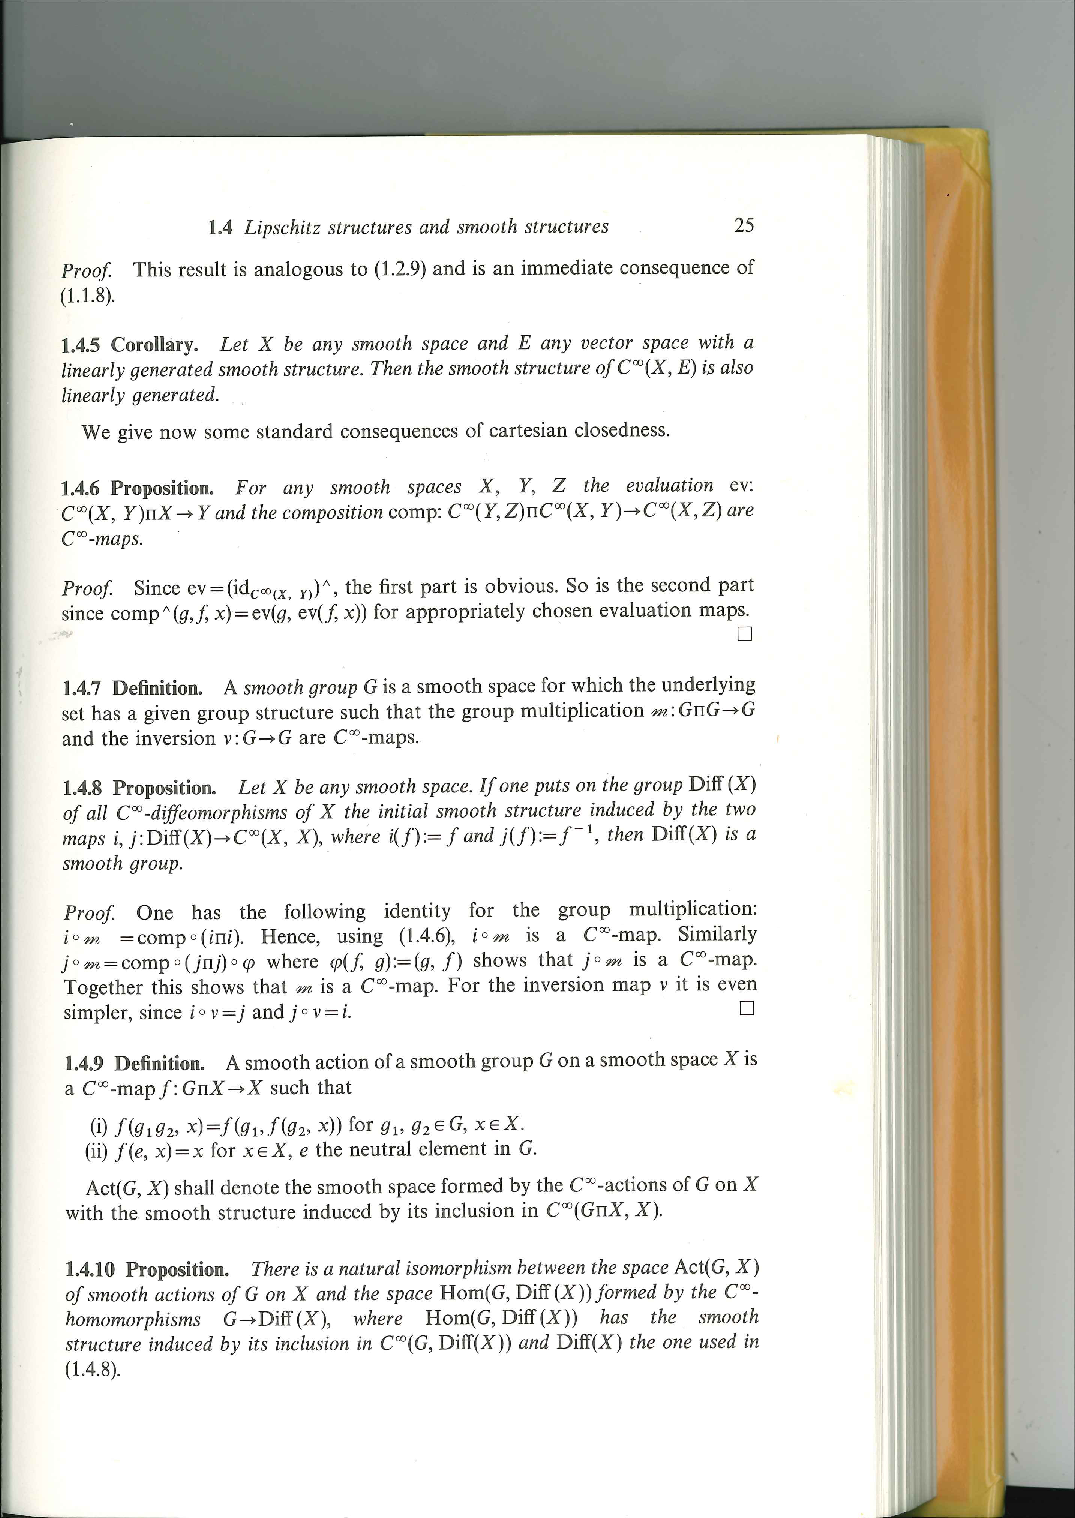
\includegraphics[width=182mm]{images/frolicher_kriegl_p25}}
}
\end{column}
\begin{column}{0.28\textwidth}
\textsmaller{
Alfred Fr\"olicher, Andreas Kriegl. \emph{Linear Spaces and Differentiation Theory}. John Wiley \& Sons. 1988.}
\end{column}
\end{columns}
\end{frame}

%--------------------------------------------------------------------
%--- Multiple columns
%--------------------------------------------------------------------

\begin{frame}
\frametitle{Multiple Columns}
\begin{center}
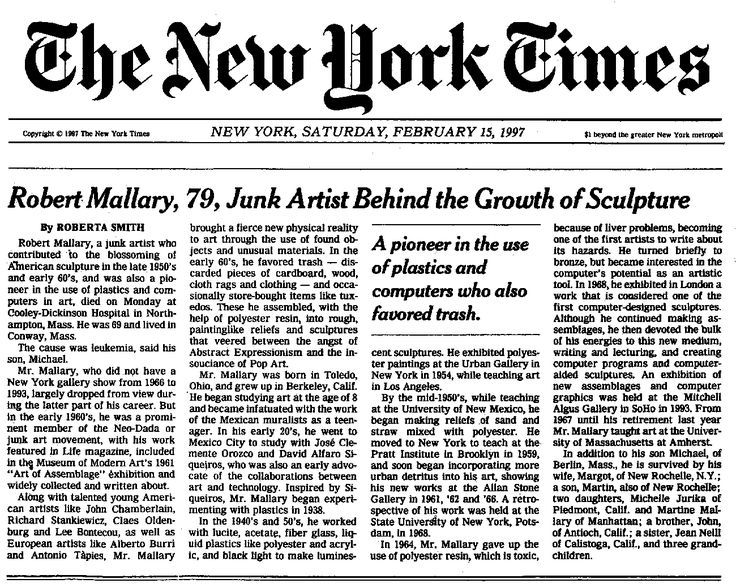
\includegraphics[width=0.83\linewidth]{images/nytimes_cover}
\end{center}
\end{frame}

%--------------------------------------------------------------------
%--- Page margins
%--------------------------------------------------------------------

\begin{frame}
\frametitle{Page Margins}
\begin{columns}
\begin{column}{0.5\textwidth}
\onslide<1->
\begin{center}
\vspace{-2em}
LibreOffice \medskip

\fbox{%
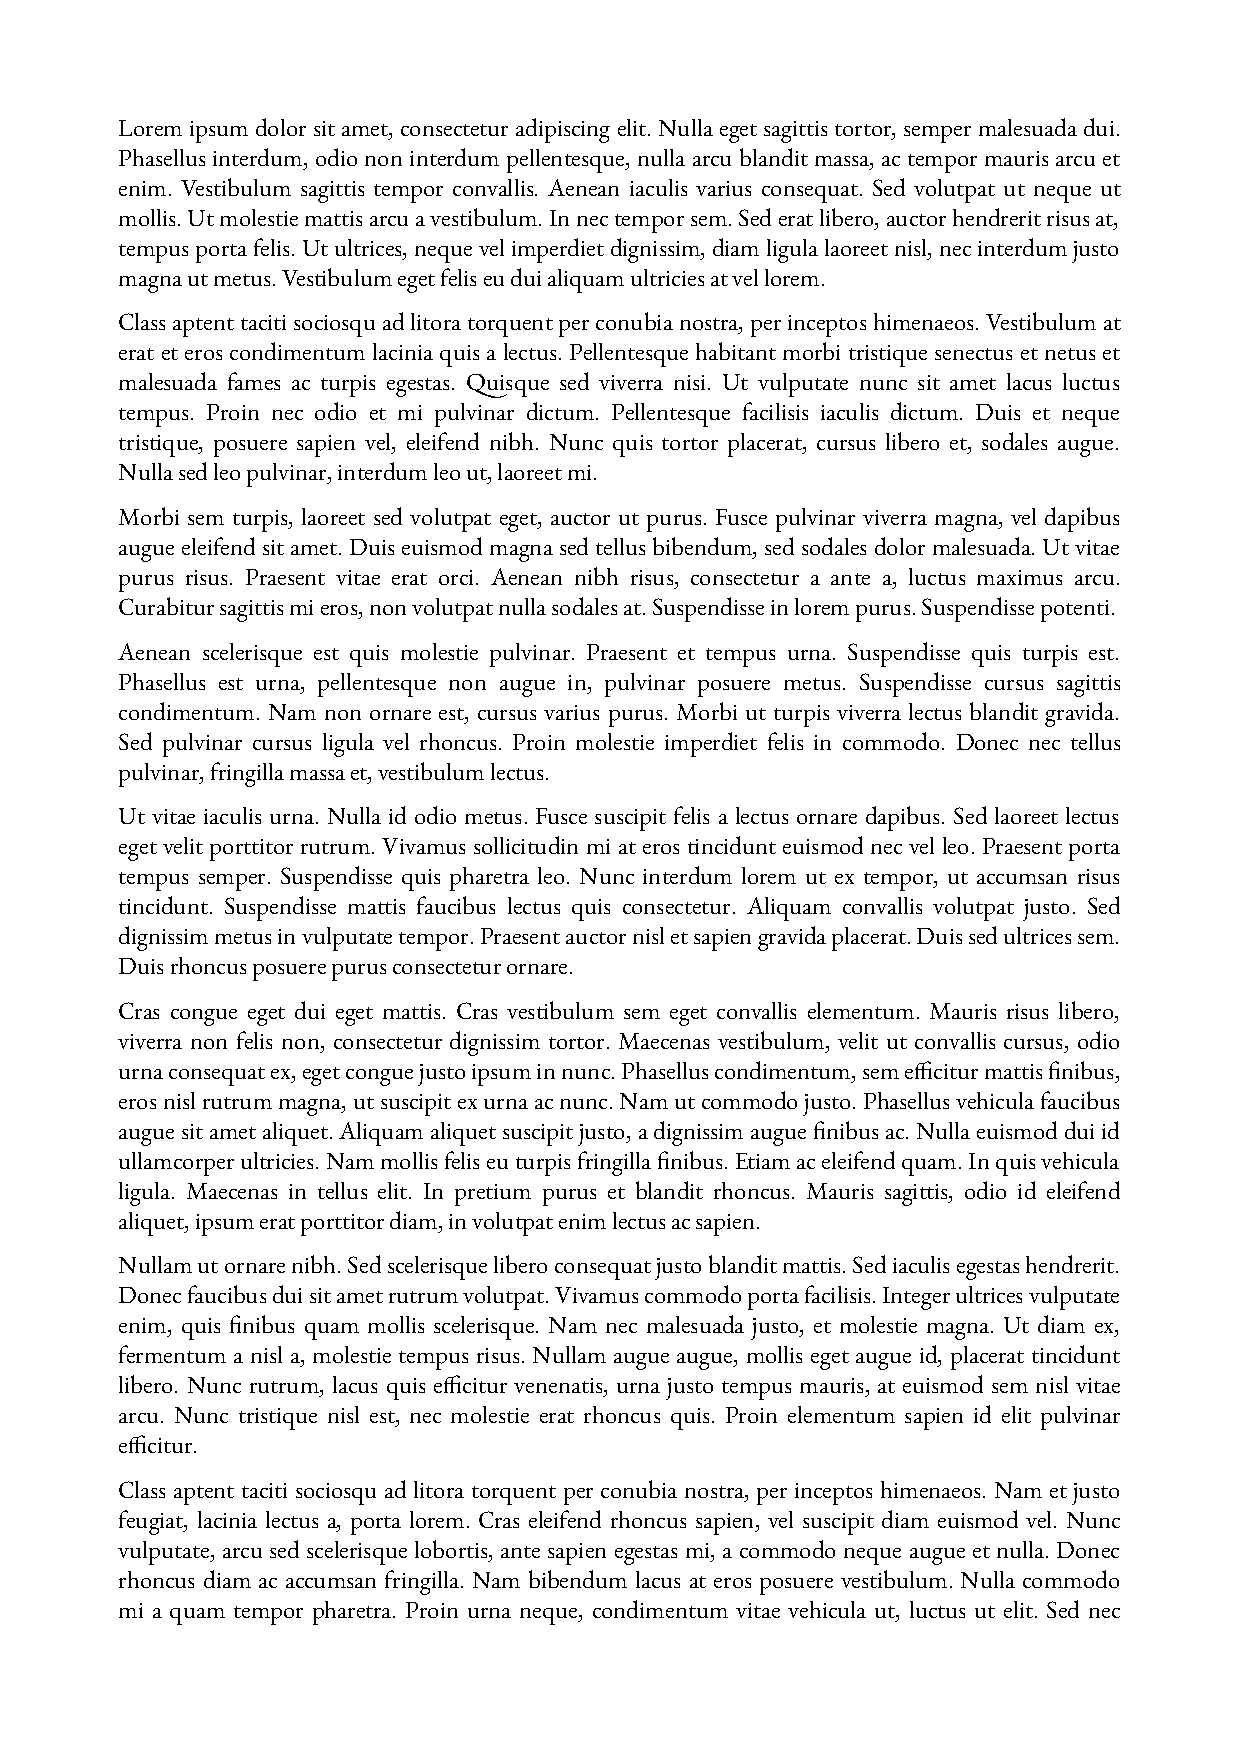
\includegraphics[width=.7\linewidth]{examples/word_lorem}
}
\end{center}

\onslide<2->
\textsmaller{Margins: L 2cm, R 2cm, T 2cm, B 2cm \\
Characters/line: 103}
\end{column}

\begin{column}{0.5\textwidth}
\onslide<1->
\begin{center}
\vspace{-2em}
\LaTeX\ article class \medskip

\fbox{%
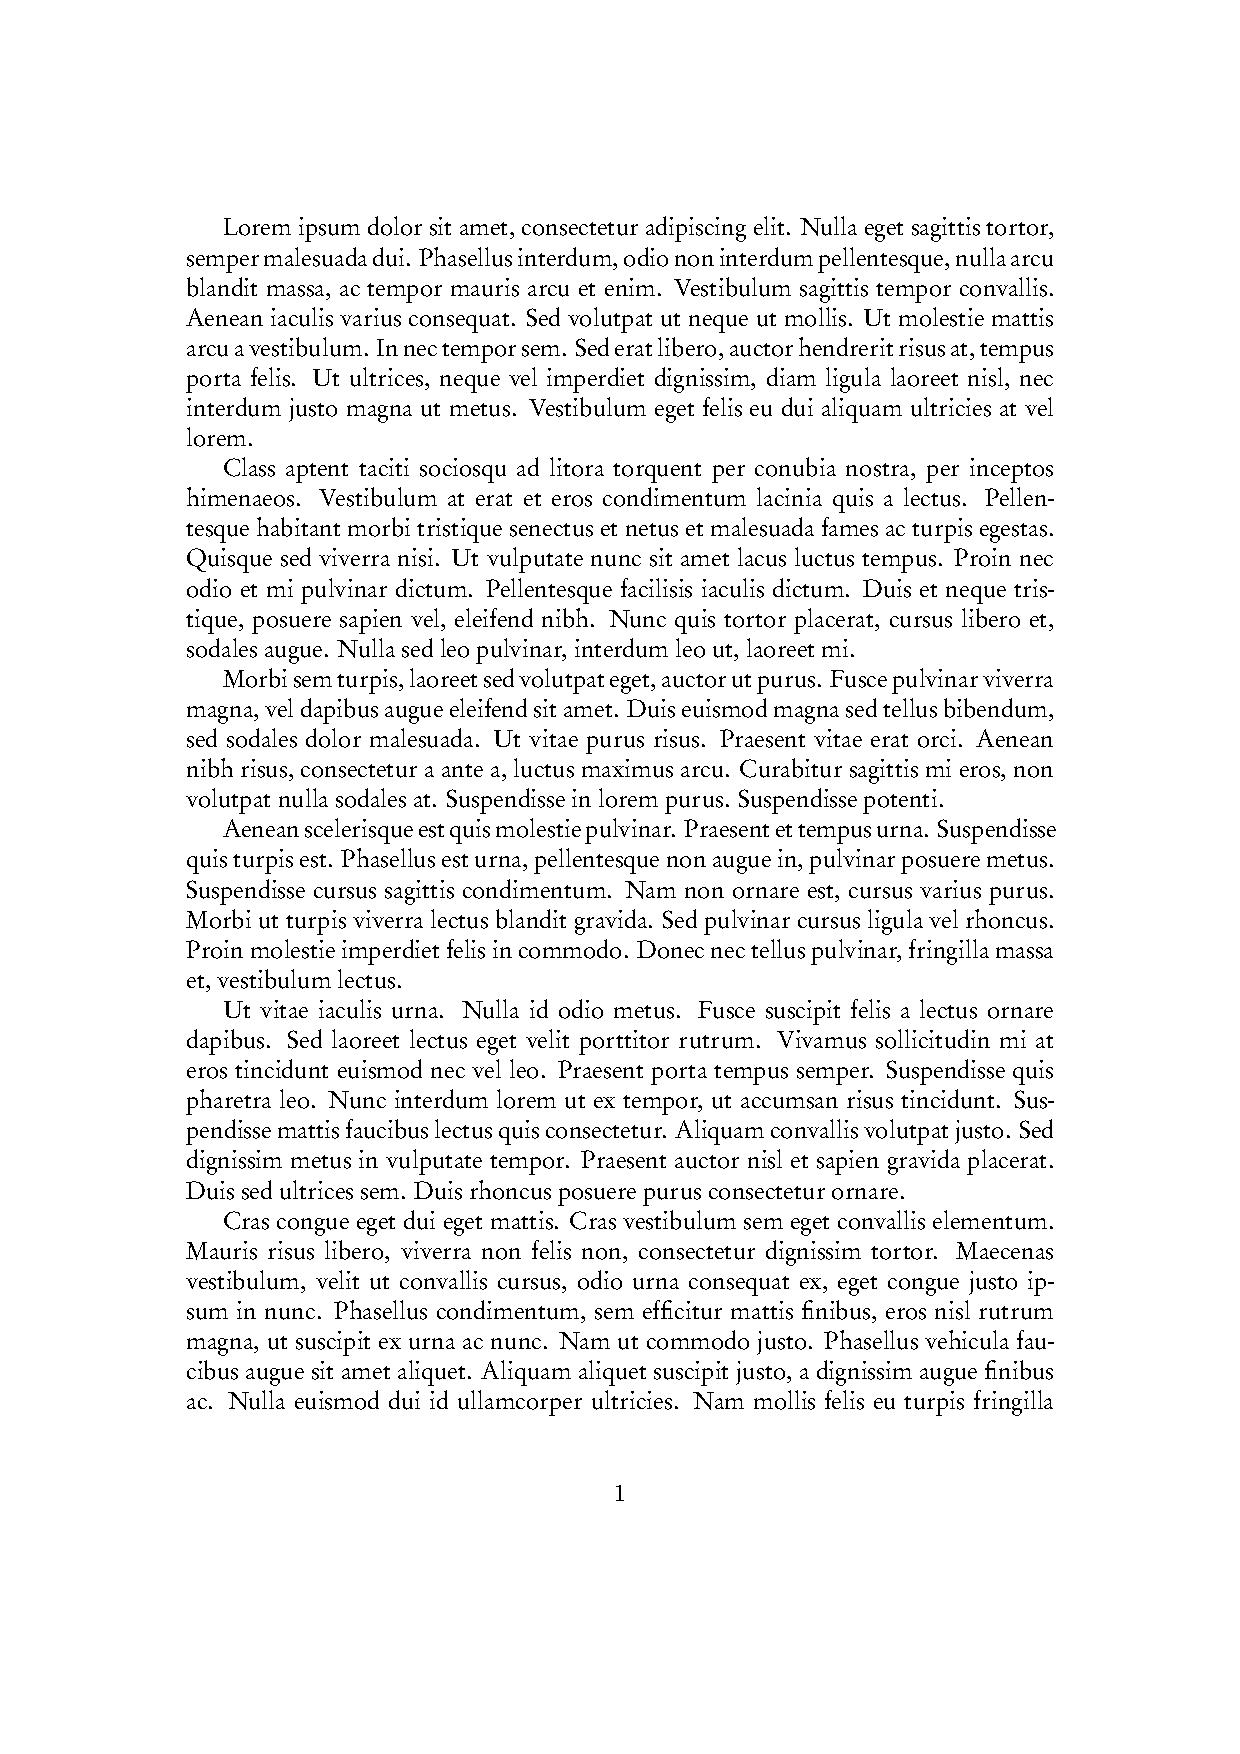
\includegraphics[width=.7\linewidth]{examples/latex_lorem}
}
\end{center}

\onslide<2->
\textsmaller{Margins: L 3cm, R 3cm, T 3.5cm, B 5.5cm \\
Characters/line: 85
}
\end{column}
\end{columns}
\end{frame}

%--------------------------------------------------------------------
%--- Book of Kells
%--------------------------------------------------------------------

\begin{frame}
\frametitle{The Book of Kells}
\begin{center}
\vspace{-1em}
\fbox{%
\adjustbox{trim={0px} {170px} {0px} {0px}, clip, scale=0.5}{%
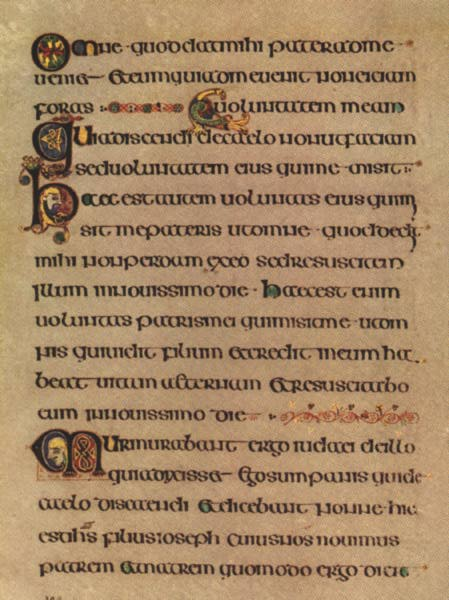
\includegraphics[width=449px]{images/book_of_kells}}
}
\end{center}
\vspace{-1em}
\hfill\footnotesize{Source: Wikimedia Commons
\href{https://commons.wikimedia.org/wiki/File:KellsFol309r.jpg}{(link)}.}
\end{frame}

%--------------------------------------------------------------------
%--- Gutenberg bible
%--------------------------------------------------------------------

\begin{frame}
\frametitle{The Gutenberg Bible}
\begin{center}
\vspace{-1em}
\fbox{%
\adjustbox{trim={0cm} {700px} {10px} {34px}, clip, scale=0.32}{%
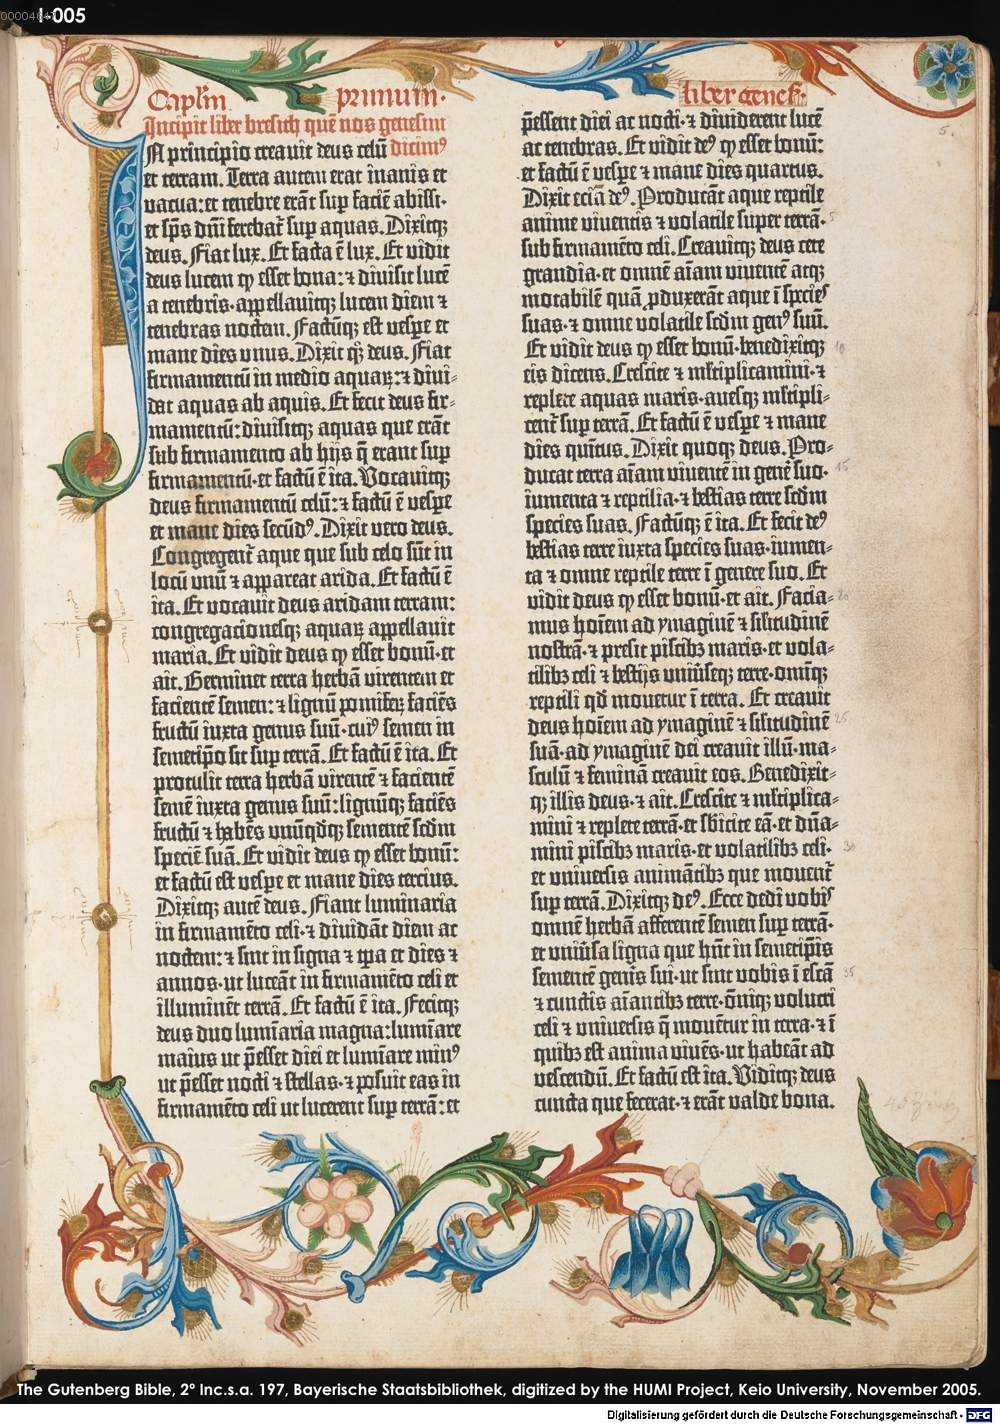
\includegraphics[width=1000px]{images/gutenberg_bible_1x}}
}
\end{center}
\vspace{-1em}
\hfill\footnotesize{Source: Bayerische Staatsbibliothek 
\href{http://daten.digitale-sammlungen.de/bsb00004647/image_13}{(link)}.}
\end{frame}

%--------------------------------------------------------------------
%--- Manual Typesetting
%--------------------------------------------------------------------

\begin{frame}
\frametitle{Manual Typesetting}
\begin{columns}[b]
\begin{column}{0.65\textwidth}
\fbox{%
\adjustbox{trim={1.8cm} {10.3cm} {2.6cm} {2cm}, clip, scale=0.7}{%
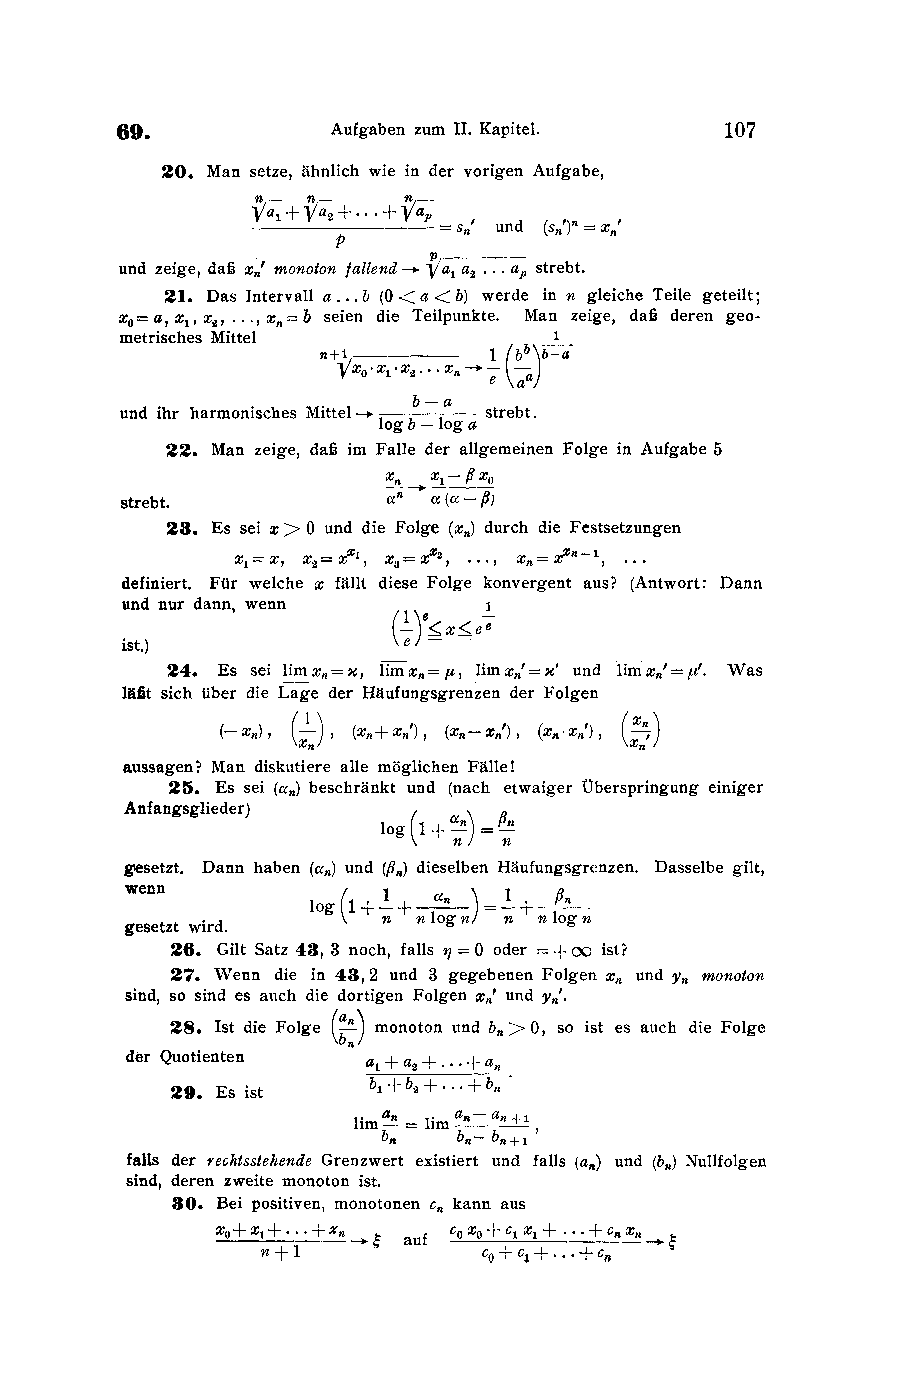
\includegraphics[width=155mm]{images/knopp_reihen_p108}}
}
\end{column}
\begin{column}{0.35\textwidth}
\textsmaller{
Konrad Knopp. \emph{Theorie und Anwendung der Unendlichen Reihen}. Zweite Auflage. Springer. 1924.}
\end{column}
\end{columns}

\end{frame}


%--------------------------------------------------------------------
%--- Written with a Typewriter
%--------------------------------------------------------------------

\begin{frame}
\frametitle{Written with a Typewriter}
\begin{columns}[b]
\begin{column}{0.6\textwidth}
\fbox{%
\adjustbox{trim={1.5cm} {3cm} {1.3cm} {6.5cm}, clip, scale=0.6}{%
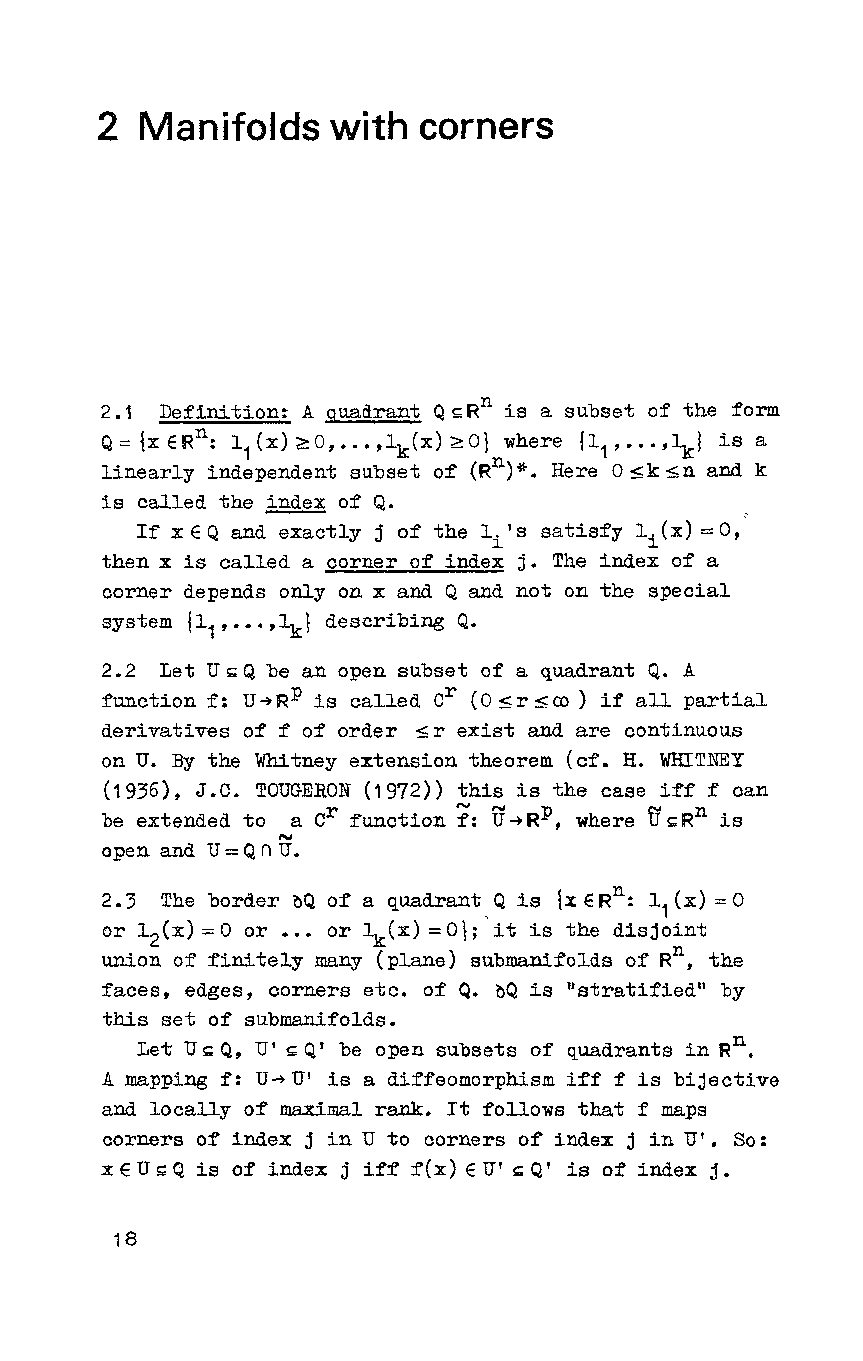
\includegraphics[width=146mm]{images/michor_shiva_p25}}
}
\end{column}
\begin{column}{0.4\textwidth}
\textsmaller{
Peter Michor. \emph{Manifolds of Differentiable Mappings}. Shiva Publishing Limited, Orpington. 1980.}
\end{column}
\end{columns}
\end{frame}

%--------------------------------------------------------------------
%--- Written by Hand
%--------------------------------------------------------------------

\begin{frame}
\frametitle{Written by Hand}
\begin{columns}[b]
\begin{column}{0.57\textwidth}
\fbox{%
\adjustbox{trim={2cm} {7.5cm} {3cm} {2.3cm}, clip, scale=0.6}{%
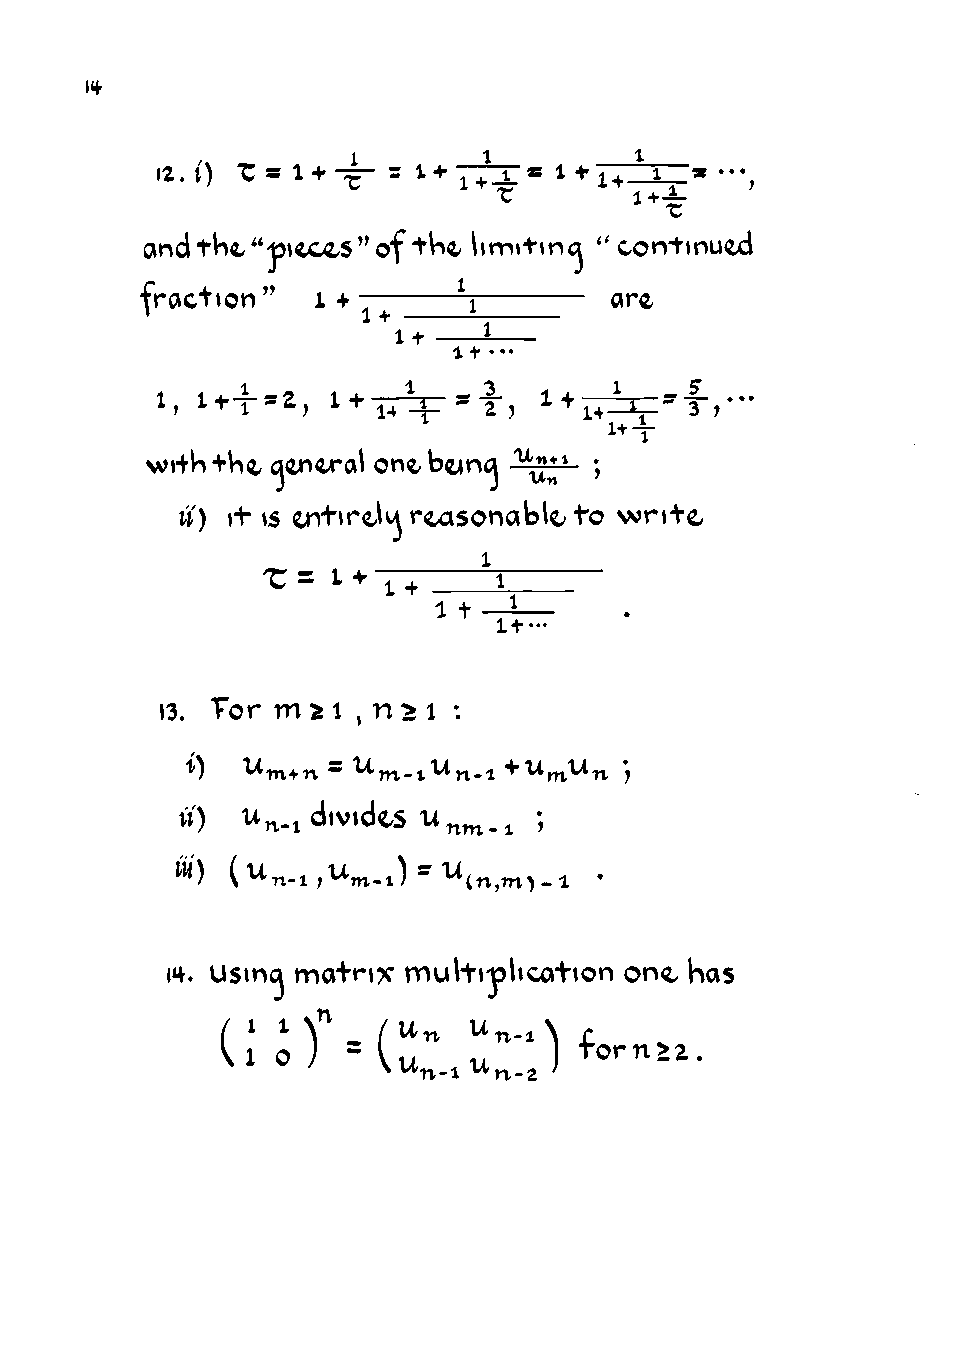
\includegraphics[width=162mm]{images/roberts_number_theory_p29}}
}
\end{column}
\begin{column}{0.43\textwidth}
\textsmaller{
Joe Roberts. \emph{Elementary Number Theory. A Problem Oriented Approach}. The MIT Press, Cambridge. 1977.}
\end{column}
\end{columns}
\end{frame}

%%% Local Variables:
%%% TeX-master: "talk"
%%% End:


%--------------------------------------------------------------------
%--- Summary
%--------------------------------------------------------------------

% \section{Wrapping Up}

% \begin{frame}
% \frametitle{Summary}
% \begin{itemize}
% \item<+-> \LaTeX
% 	\begin {itemize}
% 	\item a document preparation system
% 	\item professional quality typesetting output
% 	\end{itemize}
% \item<+-> Output types
% 	\begin{itemize}
% 	\item Final year project, reports, books
% 	\item Presentations, posters
% 	\item Domain-specific material
% 	\end{itemize}
% \item<+-> Usage scenarios
% 	\begin{itemize}
% 	\item Direct authoring of a document
% 	\item Automatic generation (via scripts etc.)
% 	\item Typesetting of key parts (e.g. graphs)
% 	\end{itemize}
% \end{itemize}
% \end{frame}

%--------------------------------------------------------------------
%--- Questions
%--------------------------------------------------------------------

\begin{frame}{The End}
\centering
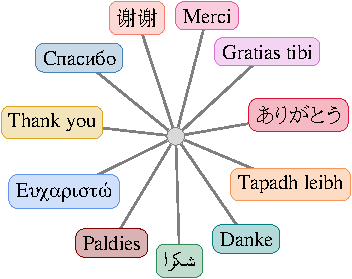
\includegraphics[width=.6\textwidth]{images/multilingual_thank_you}

\bigskip 
\begin{tabular}{cl}
\multirow{2}{*}{\LARGE Questions?} & 
Martins Bruveis (\url{martins.bruveris@brunel.ac.uk}) \\ & 
Paresh Date (\url{paresh.date@brunel.ac.uk}) \\
\end{tabular}

\end{frame}

%--------------------------------------------------------------------
%--- Licence
%--------------------------------------------------------------------

\begin{frame}
\frametitle{Licence}

\btVFill

{\huge \ccbyncsa}
\medskip

This work, \emph{\rmfamily An Introduction to \LaTeX}, is a derivative of \\
\href{https://www.overleaf.com/read/cyfvvyfrpmyn}{\emph{\structure{\LaTeX: More Than Just Academic Papers and Theses}}} by 
\href{http://liantze.penguinattack.org/}{\structure{LianTze Lim}}, used under \ccbyncsa. This work is licenced under \ccbyncsa\ by Martins Bruveris.
\bigskip
\end{frame}

%--------------------------------------------------------------------
%--- End of document
%--------------------------------------------------------------------

\end{document}

%%% Local Variables:
%%% TeX-master: t
%%% End:
